\documentclass[12pt,a4paper]{article}

% ==================== 基础宏包 ====================
\usepackage[UTF8]{ctex}
\usepackage[margin=2.2cm]{geometry}
\usepackage{amsmath,amssymb,amsthm,mathtools}
\usepackage{array}
\usepackage{booktabs}
\usepackage{enumitem}
\usepackage{xcolor}
\usepackage{graphicx}
\usepackage{fancyhdr}
\usepackage{lastpage}
\usepackage{hyperref}
\usepackage[most]{tcolorbox}
\usepackage{titlesec}
\usepackage{tabularx}
\usepackage{longtable}
\usepackage{listings}
\lstdefinestyle{rcode}{
  language=R,
  basicstyle=\ttfamily\footnotesize,
  keywordstyle=\color{mainblue},
  commentstyle=\color{textgray},
  stringstyle=\color{mainblue},
  breaklines=true,
  columns=fullflexible,
  keepspaces=true,
  showstringspaces=false,
  frame=single,
  rulecolor=\color{linegray},
  numbers=left,
  numberstyle=\tiny\color{textgray},
  xleftmargin=2em
}

\hypersetup{
  hidelinks
}

% ==================== 颜色定义 ====================
\definecolor{mainblue}{RGB}{34,72,112}
\definecolor{lightblue}{RGB}{241,246,252}
\definecolor{linegray}{RGB}{210,218,228}
\definecolor{textgray}{RGB}{90,98,108}

% ==================== 页面设置 ====================
\setlength{\parindent}{2em}
\setlength{\parskip}{0.35em}
\setlength{\headheight}{25pt}
\linespread{1.2}

\pagestyle{fancy}
\fancyhf{}
\lhead{\textcolor{textgray}{\small 高维数据分析课程作业}}
\rhead{\textcolor{textgray}{\small \thepage/\pageref*{LastPage}}}
\cfoot{}
\renewcommand{\headrulewidth}{0.4pt}
\renewcommand{\headrule}{%
  \hbox to\headwidth{\color{linegray}\leaders\hrule height \headrulewidth\hfill}}

% ==================== 标题样式 ====================
\titleformat{\section}
  {\Large\bfseries\color{mainblue}}
  {\thesection}
  {0.6em}
  {}

\titleformat{\subsection}
  {\large\bfseries\color{mainblue}}
  {\thesubsection}
  {0.6em}
  {}

\titlespacing*{\section}{0pt}{1.2em}{0.6em}
\titlespacing*{\subsection}{0pt}{0.8em}{0.4em}

% ==================== 自定义环境 ====================
\newtcolorbox{infobox}{
  colback=lightblue,
  colframe=mainblue,
  boxrule=0.6pt,
  arc=2mm,
  left=1.2em,
  right=1.2em,
  top=0.8em,
  bottom=0.8em
}

\newtcolorbox{answerbox}{
  colback=white,
  colframe=linegray,
  boxrule=0.5pt,
  arc=2mm,
  left=1em,
  right=1em,
  top=0.8em,
  bottom=0.8em,
  breakable,
  lines before break=6
}

% ==================== 作业信息 ====================
\newcommand{\course}{高维数据分析}
\newcommand{\homeworktitle}{第2次作业}
\newcommand{\studentname}{倪伟丰}
\newcommand{\studentid}{2024110089}
\newcommand{\classname}{24 大数据 2 班}
\newcommand{\teacher}{袁洪松}
\newcommand{\duedate}{2026年10月29日 22:00}
\newcommand{\totalpoints}{130}

% ==================== 正文开始 ====================
\begin{document}

\begin{center}
  {\Huge\bfseries\color{mainblue}\homeworktitle}\\[0.6em]
  {\Large\course}\\[1.2em]
  {\color{linegray}\rule{0.9\textwidth}{0.8pt}}
\end{center}

\begin{infobox}
\begin{tabularx}{\linewidth}{>{\bfseries}p{2.2cm} X >{\bfseries}p{2.2cm} X}
姓名 & \studentname & 学号 & \studentid \\
班级 & \classname & 教师 & \teacher \\
截止时间 & \duedate & 总分 & \totalpoints 分
\end{tabularx}
\end{infobox}

% ==================================================
\section{Problem 1（15 分）}

\texttt{salary.csv} 记录了某学院 52 名教师的薪资与背景信息。取年薪 \texttt{salary} 为因变量，职称 \texttt{rank} 与最高学位 \texttt{degree} 为两个分类自变量 $F_1,F_2$。

\subsection{}

统计两个因子的类别及各类别样本数。含截距时，各需引入多少个虚拟变量？（4 分）

\begin{answerbox}
\textbf{解：}
从提供的 \texttt{salary.csv} 读入数据，将职称和学位设为分类变量：
\begin{lstlisting}[style=rcode]
salary <- read.csv(file.path(data_dir, "salary.csv"))
salary$rank <- factor(salary$rank,
                      levels = c("Asst", "Assoc", "Prof"))
salary$degree <- factor(salary$degree,
                        levels = c("Masters", "PhD"))
table(salary$rank, salary$degree)
\end{lstlisting}
其中 \texttt{data\_dir} 由 \texttt{Assignment2.R} 的公共设置定位至本作业的数据目录。类别及频数为：
\begin{center}
\begin{tabular}{lrrr}
\toprule
职称 & Masters & PhD & 合计 \\
\midrule
Asst & 14 & 4 & 18 \\
Assoc & 5 & 9 & 14 \\
Prof & 15 & 5 & 20 \\
\midrule
合计 & 34 & 18 & 52 \\
\bottomrule
\end{tabular}
\end{center}
职称有 3 类，最高学位有 2 类，共 52 条记录，二者的交叉列联表无空单元格。
含截距时，为避免虚拟变量与截距完全共线，分别用 $3-1=2$ 个职称虚拟变量及 $2-1=1$ 个学位虚拟变量，连同截距共有 4 个参数。

\end{answerbox}

\subsection{}

以 \texttt{Asst}、\texttt{Masters} 为参照，写出主效应模型，估计全部系数。（7 分）
\begin{answerbox}
\textbf{解：}
本题仅使用职称与最高学位作为解释变量。以 \texttt{Asst} 和 \texttt{Masters} 为参照，定义
$$
D_i^{\mathrm{Assoc}}=I(\mathrm{rank}_i=\mathrm{Assoc}),\quad
D_i^{\mathrm{Prof}}=I(\mathrm{rank}_i=\mathrm{Prof}),\quad
D_i^{\mathrm{PhD}}=I(\mathrm{degree}_i=\mathrm{PhD}).
$$
主效应模型为
$$
Y_i=\beta_0+\beta_1D_i^{\mathrm{Assoc}}+\beta_2D_i^{\mathrm{Prof}}
+\beta_3D_i^{\mathrm{PhD}}+\varepsilon_i,\qquad i=1,\ldots,52.
$$
设 $E(\varepsilon_i\mid X)=0$、$\operatorname{Var}(\varepsilon\mid X)=\sigma^2I$；通常的精确 $t$、$F$ 检验还假定误差正态。令设计矩阵第 $i$ 行为
$(1,D_i^{\mathrm{Assoc}},D_i^{\mathrm{Prof}},D_i^{\mathrm{PhD}})$，其秩为 4，最小二乘估计为
$\hat\beta=(X^\top X)^{-1}X^\top y$。
\begin{lstlisting}[style=rcode]
fit1 <- lm(salary ~ rank + degree, data = salary)
summary(fit1)
\end{lstlisting}
\begin{center}
\small
\begin{tabular}{lrrrr}
\toprule
系数 & Estimate & Std. Error & $t$ & $p$ \\
\midrule
截距 & 17536.788 & 734.196 & 23.886 & $2.71\times10^{-28}$ \\
\texttt{rankAssoc} & 4968.348 & 1135.248 & 4.376 & $6.49\times10^{-5}$ \\
\texttt{rankProf} & 11861.298 & 970.481 & 12.222 & $2.40\times10^{-16}$ \\
\texttt{degreePhD} & 1043.455 & 940.715 & 1.109 & 0.2729 \\
\bottomrule
\end{tabular}
\end{center}
因此拟合方程为
$$
\widehat{\mathrm{salary}}_i
=17536.788+4968.348D_i^{\mathrm{Assoc}}
+11861.298D_i^{\mathrm{Prof}}+1043.455D_i^{\mathrm{PhD}}.
$$
RSS 为 $427975976.32$，残差自由度为 $52-4=48$，残差标准误为 $2985.995$；
$R^2=0.7603$，调整后 $R^2=0.7454$，整体 $F=50.76$（自由度 $3,48$，$p=6.35\times10^{-15}$）。

\end{answerbox}



\subsection{}

解释职称与学位的系数含义。若改变参照类别，拟合值与 RSS 是否改变？说明原因。（4 分）

\begin{answerbox}
\textbf{解：}
在学位相同的条件下，\texttt{Assoc} 和 \texttt{Prof} 相对于 \texttt{Asst} 的拟合期望年薪分别高 $4968.348$ 和 $11861.298$；在职称相同的条件下，\texttt{PhD} 相对于 \texttt{Masters} 的拟合期望年薪高 $1043.455$。
截距 $17536.788$ 是 \texttt{Asst}+\texttt{Masters} 组的拟合期望年薪。主效应模型未含交互，因而假定学位差异在各职称中相同。这些是模型中的条件均值差异，不能直接解释为因果效应。

若改变参照类别，拟合值与 RSS 均不改变。新的设计矩阵 $X_*$ 是 $X$ 的可逆线性重参数化，故 $\mathcal C(X_*)=\mathcal C(X)$；最小二乘投影矩阵
$$
H=X(X^\top X)^{-1}X^\top
$$
不变，因而 $\hat y=Hy$ 与 $\mathrm{RSS}=\|y-\hat y\|^2$ 不变。改变的是截距及比较系数所代表的具体对比；若用两种编码检验同一个可估对比，检验结果仍相同。

\end{answerbox}

% ==================================================
\section{Problem 2（10 分）}

\texttt{wblake.csv} 包含 439 条小口黑鲈的测量记录，\texttt{Length} 为捕获时鱼长（mm），\texttt{Scale} 为鱼鳞半径（mm）。取 $Y=\texttt{Length}$、$x=\texttt{Scale}$。

\subsection{}

分别拟合 1 至 5 阶多项式回归，报告系数、RSS 与调整后的 $R^2$，在散点图上叠加拟合曲线（按 $x$ 排序或用等距网格绘图）。可用正交多项式，但应注明基底。（6 分）

\begin{answerbox}
\textbf{解：}

$d$ 阶多项式回归模型为：

$$
y_i=\beta_0 +\sum_{j=1}^{d} \beta_j x_i^j + \varepsilon_i
$$

采用原始幂基底（\texttt{poly(Scale, d, raw=TRUE)}），即 $y_i=\beta_0+\sum_{j=1}^{d}\beta_j x_i^j+\varepsilon_i$，$n=439$。

\textbf{R代码：}
\begin{lstlisting}[style=rcode]
wblake <- read.csv(file.path(data_dir, "wblake.csv"))
fits <- lapply(1:5, function(d) lm(Length ~ poly(Scale, d, raw = TRUE), data = wblake))
\end{lstlisting}

\textbf{系数估计：}
\begin{center}
\small
\begin{tabular}{lrrrrr}
\toprule
系数 & 1 阶 & 2 阶 & 3 阶 & 4 阶 & 5 阶 \\
\midrule
截距 & 56.29860124 & 15.32341499 & 15.21866002 & 11.05977492 & -6.63103638 \\
$x$ & 23.30683403 & 39.31259046 & 39.37338298 & 42.76364613 & 61.91580632 \\
$x^2$ & --- & -1.27104257 & -1.28081601 & -2.16532147 & -9.26592312 \\
$x^3$ & --- & --- & 0.00046254 & 0.09041200 & 1.24372376 \\
$x^4$ & --- & --- & --- & -0.00308051 & -0.08729638 \\
$x^5$ & --- & --- & --- & --- & 0.00225293 \\
\bottomrule
\end{tabular}
\end{center}

\textbf{RSS 与调整后 $R^2$：}
\begin{center}
\small
\begin{tabular}{lccccc}
\toprule
 & 1 阶 & 2 阶 & 3 阶 & 4 阶 & 5 阶 \\
\midrule
RSS & 232405.7 & 189849.1 & 189849.0 & 189796.8 & 189468.5 \\
调整后 $R^2$ & 0.8808 & 0.9024 & 0.9022 & 0.9020 & 0.9019 \\
\bottomrule
\end{tabular}
\end{center}

\begin{center}
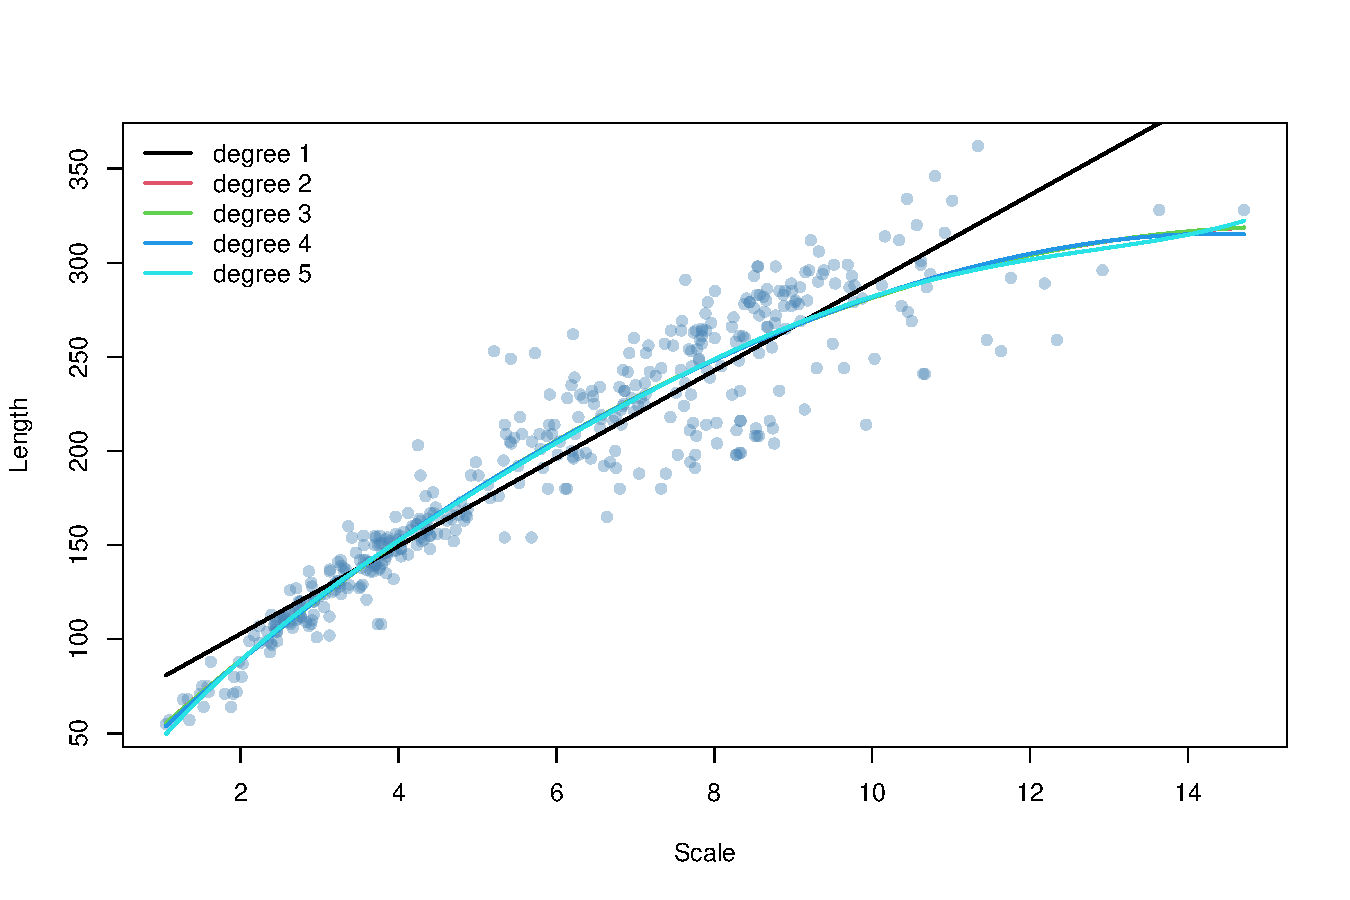
\includegraphics[width=0.65\textwidth]{assets/r-results/problem2-poly-fits.pdf}
\\{\small\color{textgray} 图：散点与 1--5 阶多项式拟合曲线（等距网格预测并按 x 排序连线）}
\end{center}

从 1 阶增加到 2 阶后，RSS 明显下降，调整后 $R^2$ 从 $0.8808$ 升至 $0.9024$，说明加入曲率项改善了样本内拟合。2--5 阶曲线在大部分区间接近，高阶项仅带来较小的 RSS 下降，而调整后 $R^2$ 逐步下降；这些结果支持采用较低阶模型，但没有独立验证误差，不能据此断定高阶模型已经过拟合。上表保留较多小数，因为高次幂会放大系数的舍入误差；作图与预测均使用未舍入的拟合对象。

\textbf{如果采用正交多项式，则拟合模型变为：}
$$
y_i=\gamma_0+\sum_{j=1}^{d}\gamma_j P_j(x_i)+\varepsilon_i,
\quad i=1,\dots,n,\ n=439,
$$
其中 $x_i$ 为 \texttt{Scale}，$y_i$ 为 \texttt{Length}，$P_j(\cdot)$ 为恰为 $j$ 次的多项式（首项系数取正），满足以样本为内积的经验规范正交条件：
$$
\sum_{i=1}^{n}P_j(x_i)=0,\qquad
\sum_{i=1}^{n}P_j(x_i)P_k(x_i)=\delta_{jk}
=\begin{cases}1,&j=k,\\ 0,&j\ne k,\end{cases}
\quad 1\le j,k\le d.
$$
即含截距的设计矩阵 $[1,P_1,\dots,P_d]$ 列两两正交：截距列与每个 $P_j$ 正交（故 $P_j$ 已中心化），$P_j$ 之间相互正交且平方和为 1。

根据代码 \texttt{poly(Scale, d, raw=FALSE)}（即 \texttt{raw=FALSE} 的默认正交模式），选择的基底是\textbf{由本次观测到的 \texttt{Scale} 经验分布经三项递推构造出的规范正交多项式基}，而非固定的单项式 $1,x,\dots,x^d$。具体地，$P_j$ 可写成 $1,x,\dots,x^j$ 的线性组合，但组合系数由样本决定，并保存在 \texttt{attr(., "coefs")} 的 \texttt{alpha}（中心化常数）与 \texttt{norm2}（归一化常数）中；换一批 $x$ 数据，同一符号 $P_j(\cdot)$ 的函数形式也会改变。它的一个直接推论是截距 $\hat{\gamma}_0=\bar{y}$（本例中恒为 $192.97$），且对所有 $j=1,\ldots,d$，正规方程给出 $\hat{\gamma}_j=\sum_i P_j(x_i)y_i$；在误差协方差为 $\sigma^2I$ 的假设下，各斜率估计互不相关。

\textbf{R代码：}将 \texttt{raw} 的参数设置为 \texttt{FALSE}
\begin{lstlisting}[style=rcode]
fits_Orthogonality <- lapply(1:5, function(d) lm(Length ~ poly(Scale, d, raw=FALSE), data=wblake))                                                                                 
\end{lstlisting}

正交基（\texttt{raw=FALSE}）与原始幂基（\texttt{raw=TRUE}）在\textbf{拟合层面完全一致}，
在\textbf{参数化层面不一致}。一致的是：拟合值 $\hat{y}_i$、残差、RSS、$R^2$／调整后 $R^2$、整体 $F$ 检验、
在等距网格上的预测曲线；不一致的是：回归系数的数值、标准误及其单个 $t$ 检验（最高阶项的 $\lvert t\rvert$ 除外，
它在两种参数化下相同，例如 $d=2$ 时 $x^2$ 项与 $P_2$ 项的 $t$ 均为 $-9.886$）。

原因：对固定阶数 $d$，两组基张成\textbf{同一个列空间}，即次数不超过 $d$ 的全体多项式空间
$\mathcal{P}_d=\mathrm{span}\{1,x,\dots,x^d\}=\mathrm{span}\{1,P_1,\dots,P_d\}$。
正交基只是对原始幂基做了一个依赖于样本的可逆线性变换（上三角矩阵），故设计矩阵满足
$\mathcal{C}(X_{\mathrm{orth}})=\mathcal{C}(X_{\mathrm{raw}})$，最小二乘投影
$\hat{y}=X(X^{\top}X)^{-1}X^{\top}y$ 不变，从而 $\mathrm{RSS}=\lVert y-\hat{y}\rVert^2$、
调整后 $R^2$ 与预测曲线都不变；改变的只是坐标 $\hat{\beta}=(X^{\top}X)^{-1}X^{\top}y$。
经核对，$d=1,\dots,5$ 时两种写法的 RSS 与调整后 $R^2$ 在小数点后 4 位完全相同
（如 $d=2$ 时 RSS 均为 $189849.06$，调整后 $R^2$ 均为 $0.9024$），拟合值向量最大差 $<5\times 10^{-12}$（纯数值舍入），
故两组曲线在图上完全重合。实际意义：正交基下 $X^{\top}X$ 为对角阵，在球形误差假设下估计互不相关，通常也更利于数值计算。原始幂基便于写出函数表达式，但各幂次项由同一个 $x$ 决定，不能把 $\beta_j$ 解释为保持其他幂次不变时 $x$ 的边际效应。实际斜率为
$$
\frac{d\hat f(x)}{dx}=\sum_{j=1}^{d}j\hat\beta_jx^{j-1}.
$$

\end{answerbox}

\subsection{}

用 BIC 选择阶数，结合曲线解释选择结果，并说明为什么不能仅凭训练 RSS 选模型。（4 分）

\begin{answerbox}
\textbf{解：}

\textbf{R 代码：}
\begin{lstlisting}[style=rcode]
fits <- lapply(1:5, function(d) lm(Length ~ poly(Scale, d, raw = TRUE), data = wblake))
for (d in 1:5) {
  print(BIC(fits[[d]]))
}
\end{lstlisting}

\begin{center}
\small
\begin{tabular}{lccccc}
\toprule
 & 1 阶 & 2 阶 & 3 阶 & 4 阶 & 5 阶 \\
\midrule
BIC & 4017.38 & \textbf{3934.67} & 3940.75 & 3946.72 & 3952.04 \\
\bottomrule
\end{tabular}
\end{center}

BIC 以 2 阶为最小，故选择 $d=2$。这与散点叠加曲线一致：1 阶直线明显欠拟合，
未能描述拟合曲线的弯曲趋势；2 阶抛物线已刻画出数据的特征，而 3-5 阶曲线与 2 阶几乎重合，
仅在右端边界有轻微摆动，对 RSS 的改进微乎其微（2 阶到 5 阶 RSS 仅下降约 $380$），
却分别多付出 $\log n$、$2\log n$、$3\log n$ 的复杂度惩罚，故 BIC 反而回升；调整后 $R^2$ 同样在 2 阶达到最大 $0.9024$，
佐证了 2 阶的简约性。

不能仅凭训练 RSS 选模型，因为高阶模型列空间包含低阶模型列空间，
训练 RSS 随 $d$ 单调非增，越大越复杂的模型拟合值只会更贴近训练样本，5阶模型的$\mathrm{RSS}$一定是最小的。
但这无法反映泛化误差，可能把样本中的噪声也拟合进去，
从而增加过拟合风险。
令 $q=d+1$ 为回归参数个数（含截距）。上表调用的是 R 的 \texttt{BIC(lm)}，还计入误差方差参数和正态似然常数：
$$
\mathrm{BIC}_{R}=n\log(\mathrm{RSS}/n)+(q+1)\log n+n\{1+\log(2\pi)\}.
$$
它与第 5、6 题采用的简化式 $n\log(\mathrm{RSS}/n)+q\log n$ 相差共同常数
$\log n+n\{1+\log(2\pi)\}=1251.913$，不影响同一样本上的模型排序。
例如二阶模型的简化 BIC 为 $2682.757$，加上该常数即上表的 $3934.670$。
\end{answerbox}

% ==================================================
\section{Problem 3（20 分）}

仍使用 \texttt{wblake.csv}，取 \texttt{Length} 为因变量、\texttt{Scale} 为自变量。

\subsection{}

分别拟合三次多项式、三次回归样条、自然三次样条和平滑样条。两个回归样条的内部结点取 \texttt{Scale} 的 25\%、50\%、75\% 分位数，边界结点取其最小值与最大值；平滑样条用 GCV 选择平滑参数。（10 分）

\begin{answerbox}
\textbf{解：}设 $x_i=\texttt{Scale}$，$y_i=\texttt{Length}$，$n=439$。四种方法都是``基展开 $+$ 最小二乘（或惩罚最小二乘）''，区别在于基函数空间以及是否施加平滑惩罚。

\textbf{(a) 三次多项式。}全局单组三次：
$$
y_i=\beta_0+\beta_1 x_i+\beta_2 x_i^2+\beta_3 x_i^3+e_i.
$$
设计矩阵为 $[1,x,x^2,x^3]$，共 4 列（含截距），OLS 估计。对应 Problem 2 中 $d=3$ 的 \texttt{raw=TRUE} 拟合。
\begin{lstlisting}[style=rcode]
fit3_poly3 <- lm(Length ~ poly(Scale, 3, raw = TRUE), data = wblake)
\end{lstlisting}

\textbf{(b) 三次回归样条。}在 $(a,b)$ 内取 $K=3$ 个内部结点 $\xi_1<\xi_2<\xi_3$，
每段区间内为三次多项式，且在结点处函数值、一阶、二阶导数连续（$C^2$ 拼接）。截断幂表示为
$$
f(x)=\beta_0+\beta_1 x+\beta_2 x^2+\beta_3 x^3
+\sum_{k=1}^{K}\beta_{k+3}(x-\xi_k)_+^3,\quad
(x-\xi)_+=\max(x-\xi,0),
$$
共 $K+4=7$ 个参数，结点固定后仍用 OLS。\texttt{bs()} 是与截断幂基张成同一空间、数值更稳定的 B 样条实现。
内部结点取 \texttt{Scale} 的 25\%、50\%、75\% 分位数，边界结点取最小值与最大值：
$$
\xi=(3.571,\ 5.786,\ 8.018),\quad (a,b)=(1.054,\ 14.710).
$$
\begin{lstlisting}[style=rcode]
library(splines)
kn <- quantile(wblake$Scale, c(0.25, 0.50, 0.75))  # 3.571 5.786 8.018
fit3_bs <- lm(Length ~ bs(Scale, knots = kn,
                          Boundary.knots = range(wblake$Scale),
                          degree = 3), data = wblake)
\end{lstlisting}

\textbf{(c) 自然三次样条。}在 (b) 基础上施加自然边界条件 $f''(a)=f''(b)=0$，并在边界结点之外（$x<a$ 或 $x>b$）作线性延拓。这里 $a=1.05423$、$b=14.70970$；$\xi_1,\xi_3$ 是内部结点，不是线性延拓的起点。边界之间仍为分段三次函数。\texttt{ns()} 直接实现该约束基（自然样条本身即三次，无需 \texttt{degree} 参数），
结点取法与 (b) 相同。
\begin{lstlisting}[style=rcode]
fit3_ns <- lm(Length ~ ns(Scale, knots = kn,
                          Boundary.knots = range(wblake$Scale)), data = wblake)
\end{lstlisting}

\textbf{(d) 平滑样条。}不预设结点个数，直接求解带惩罚的目标
$$
\min_{f}\left[\sum_{i=1}^{n}\{y_i-f(x_i)\}^2+\lambda\int \{f''(x)\}^2\,dx\right],
\quad\lambda>0,
$$
$\int(f'')^2$ 罚``不光滑''，$\lambda\to 0$ 退化为插值，$\lambda\to\infty$ 逼向直线。
理论解可表示为以各个不同观测 $x$ 为结点的自然三次样条，光滑程度由 $\lambda$ 控制。本例 439 个 $x$ 均不同，$\lambda\to0$ 时可趋于插值；若有相同 $x$ 对应不同 $y$，则不能逐点插值所有响应。
实际调用 \texttt{smooth.spline()} 时保留默认 \texttt{all.knots=FALSE}：软件从 439 个不同 $x$ 中取 114 个结点位置，在较小基空间中作惩罚拟合。以下报告这一默认实现的结果，不将其误写为使用了全部结点。
\texttt{smooth.spline} 中 \texttt{cv=FALSE} 即用 GCV 选择 $\lambda$（\texttt{cv=TRUE} 反为 LOOCV）。
\begin{lstlisting}[style=rcode]
fit3_ss <- smooth.spline(wblake$Scale, wblake$Length,
                         cv = FALSE, all.knots = FALSE)
\end{lstlisting}
GCV 结果：有效自由度 $\mathrm{df}=18.22213$，软件内部参数 $\lambda=4.738082\times10^{-5}$，\texttt{spar}=0.753864，GCV 准则值 $436.1108$。这里的 $\lambda$ 是软件对自变量区间缩放后采用的内部尺度，不能直接与原始 $x$ 尺度的惩罚系数混同。
对固定 $\lambda$，写作 $\hat y=S_\lambda y$，则 $\mathrm{df}=\operatorname{tr}(S_\lambda)$，本例的 GCV 为
$$
\operatorname{GCV}(\lambda)=\frac{\mathrm{RSS}(\lambda)/439}{\{1-\operatorname{tr}(S_\lambda)/439\}^2}.
$$

四种拟合的 $2\times 2$ 分面板如下（散点 $+$ 各自曲线，等距网格 $300$ 点预测连线）：

\begin{center}
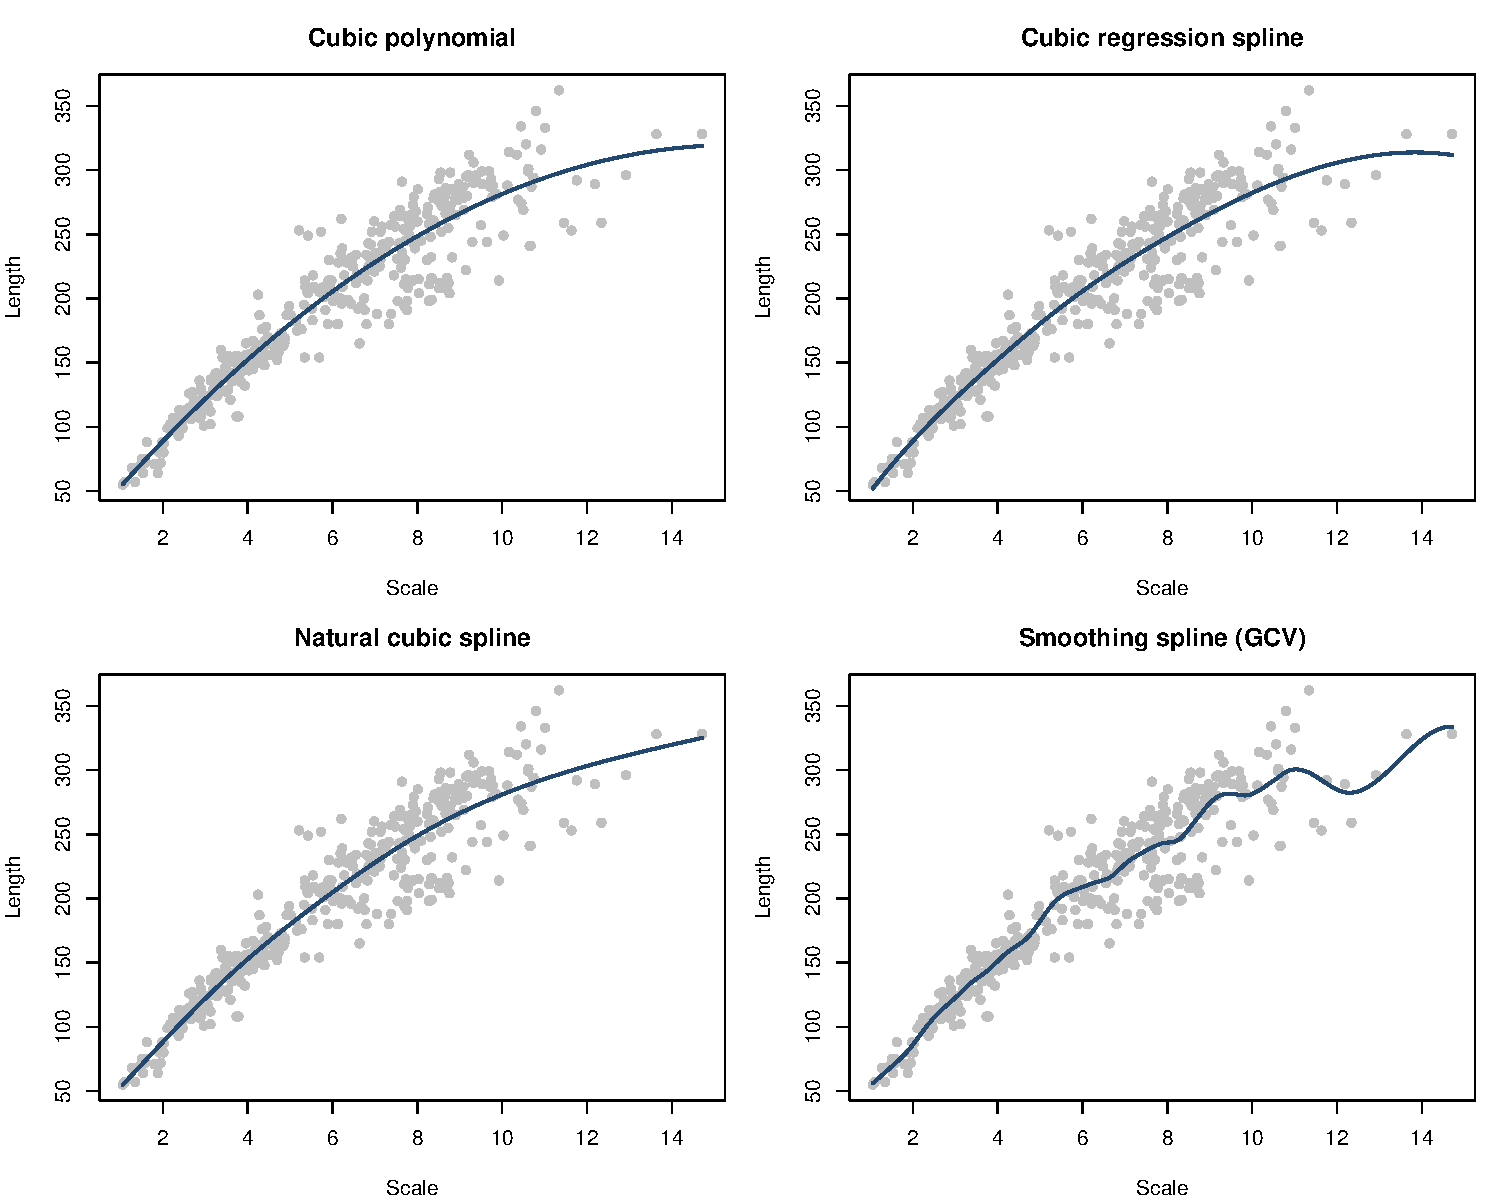
\includegraphics[width=0.8\textwidth]{assets/r-results/problem3-panels.pdf}
\\{\small\color{textgray} 图：左上三次多项式，右上三次回归样条，左下自然三次样条，右下 GCV 平滑样条}
\end{center}

\end{answerbox}

\subsection{}

在同一横轴范围内展示四条拟合曲线，报告 RSS；报告两类回归样条设计矩阵的列数（含截距）与平滑样条的有效自由度。结合曲线讨论灵活性与边界行为，并解释 RSS 最小是否足以说明模型最好。（10 分）

\begin{answerbox}
\textbf{解：}

\begin{center}
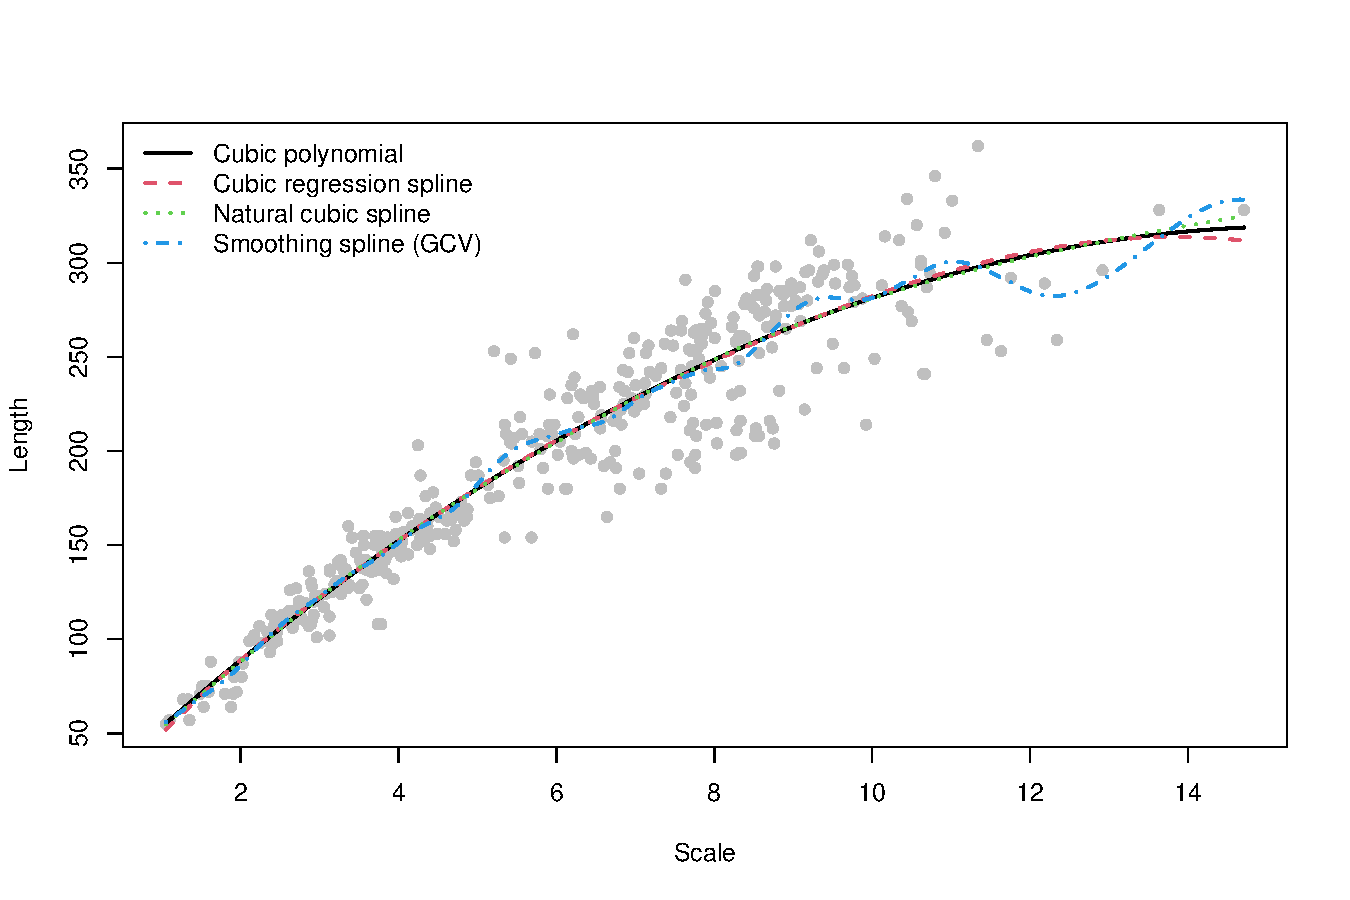
\includegraphics[width=0.7\textwidth]{assets/r-results/problem3-combined.pdf}
\\{\small\color{textgray} 图：四种拟合在同一坐标下的对比，中段几乎重合，差异集中在右端边界}
\end{center}

\begin{center}
\small
\resizebox{\linewidth}{!}{%
\begin{tabular}{lcccc}
\toprule
 & 三次多项式 & 三次回归样条 & 自然三次样条 & 平滑样条 (GCV) \\
\midrule
RSS & 189849.0 & 189662.8 & 190131.1 & \textbf{175888.7} \\
设计矩阵列数（含截距） & 4 & 7 & 5 & --- \\
有效自由度 & 4 & 7 & 5 & 18.22 \\
\bottomrule
\end{tabular}%
}
\end{center}
列数说明：三次多项式 $[1,x,x^2,x^3]$ 为 4 列；三次回归样条 $K+4=7$ 列
；自然样条施加两条独立边界约束，维数由 7 降为 5。普通最小二乘的帽子矩阵是投影矩阵，其迹等于设计矩阵秩，所以前三种方法的有效自由度分别为 4、7、5（均含截距）。平滑样条虽也有基矩阵，但惩罚使其复杂度不能直接用基函数个数表示，应使用 $\operatorname{tr}(S_\lambda)=18.22$。

四条曲线在数据密集的中段几乎重合，说明主趋势在这四个模型中都可以被学习到；
差异集中在右端边界：三次多项式中局部抖动会传导到全局，边界容易出现上翘或下坠；
三次回归样条分段拟合，内部灵活但边界仍为三次，可能在边界外产生较强弯曲；
自然样条在边界外线性延拓，限制了外推曲率，但并不保证外推误差更小。平滑样条的 $\lambda$ 由 GCV 选择，
本例 $\mathrm{df}=18.22$ 高于其余三者的有效自由度（4、7、5，均含截距），曲线最贴合局部起伏，RSS 最小（$175889$，比其余低约 $7\%$）。

\textbf{RSS 最小不足以说明最好：}RSS 是训练误差，
平滑样条用 $18.22$ 个有效自由度换来 RSS 最小，在这四种拟合中样本内误差最小，但这并不等于泛化误差最小。应使用同一验证方案（例如相同分折的 CV）比较预测误差；其中平滑样条的平滑参数也应在训练部分选择。对于未惩罚的有限维回归，可按同一口径比较 AIC/BIC；若将平滑样条纳入信息准则比较，需要明确有效自由度及似然口径，不能直接以基函数个数作为参数数目。
\end{answerbox}

% ==================================================
\section{Problem 4（10 分）}

\texttt{ais.csv} 记录了 202 名运动员的身体测量及血液指标。取体脂百分比 \texttt{Bfat} 为因变量，自变量仅使用
\[
  \texttt{Ht, Wt, BMI, RCC, WCC, Hc, Hg, Ferr, SSF}.
\]
其中 \texttt{Ht, Wt, BMI} 为身高、体重、身体质量指数；\texttt{RCC, WCC, Hc, Hg, Ferr} 为血液指标；\texttt{SSF} 为皮褶厚度总和。

\subsection{}

对九个自变量中心化并按样本标准差标准化，计算前三个主成分的载荷、各自及累计解释方差比例。说明为什么此处需要标准化。（5 分）

\begin{answerbox}
\textbf{解：}

\begin{lstlisting}[style=rcode]
ais <- read.csv(file.path(data_dir, "ais.csv"))
vars <- c("Ht", "Wt", "BMI", "RCC", "WCC", "Hc", "Hg", "Ferr", "SSF")
X <- ais[, vars]
# 中心化 + 按样本标准差标准化后做 PCA
pca <- prcomp(X, center = TRUE, scale. = TRUE)
# 前三个主成分的载荷（特征向量）
round(pca$rotation[, 1:3], 4)
# 各自及累计解释方差比例
summary(pca)$importance[, 1:3]  
\end{lstlisting}

对第 $j$ 列定义 $z_{ij}=(x_{ij}-\bar x_j)/s_j$，其中 $s_j$ 为样本标准差。令 $Z$ 为标准化矩阵，
$$
R=\frac{Z^\top Z}{201},\qquad Ru_k=\lambda_ku_k,\qquad
u_k^\top u_k=1,\qquad t_k=Zu_k.
$$
按特征值从大到小排序，$u_k$ 是载荷，$t_k$ 是得分，方差比例为 $\lambda_k/\sum_j\lambda_j=\lambda_k/9$。

\textbf{载荷（特征向量 $u_1,u_2,u_3$，符号整体翻转视为同一主成分）：}
\begin{center}
\small
\begin{tabular}{lrrr}
\toprule
变量 & PC1 & PC2 & PC3 \\
\midrule
\texttt{Ht} & $-0.3082$ & $0.2340$ & $-0.4473$ \\
\texttt{Wt} & $-0.3745$ & $0.4353$ & $-0.2293$ \\
\texttt{BMI} & $-0.3020$ & $0.4720$ & $0.0366$ \\
\texttt{RCC} & $-0.4344$ & $-0.2451$ & $0.0471$ \\
\texttt{WCC} & $-0.1125$ & $0.1625$ & $0.7447$ \\
\texttt{Hc} & $-0.4484$ & $-0.2545$ & $0.0423$ \\
\texttt{Hg} & $-0.4524$ & $-0.2250$ & $0.0527$ \\
\texttt{Ferr} & $-0.2098$ & $0.0581$ & $0.4083$ \\
\texttt{SSF} & $0.1499$ & $0.5724$ & $0.1339$ \\
\bottomrule
\end{tabular}
\end{center}
解读：PC1 是红细胞相关（\texttt{RCC,Hc,Hg}）与体型（\texttt{Ht,Wt,BMI}）的同向加权综合指标；
PC2 主要载荷在 \texttt{SSF}（$0.57$）、\texttt{BMI}（$0.47$）、\texttt{Wt}（$0.44$）上，可理解为``体脂体型''方向；
PC3 主要载荷在 \texttt{WCC}（$0.74$）与 \texttt{Ht}（$-0.45$）、\texttt{Ferr}（$0.41$）上。

\textbf{解释方差比例：}
\begin{center}
\small
\begin{tabular}{lccc}
\toprule
 & PC1 & PC2 & PC3 \\
\midrule
标准差 & $1.9973$ & $1.3872$ & $1.0193$ \\
各自解释比例 & $0.4433$ & $0.2138$ & $0.1155$ \\
累计解释比例 & $0.4433$ & $0.6571$ & $0.7725$ \\
\bottomrule
\end{tabular}
\end{center}
即 9 个标准化变量的总方差为 9，前三个特征值约为 $3.99$、$1.92$、$1.04$，前三个主成分共保留标准化自变量总方差的 $77.25\%$。

\textbf{为什么此处需要标准化：}

本题要求标准化；从分析目的看也适合如此处理，因为九个变量量纲与数量级差异极大：\texttt{Ferr} 标准差约 $47.5$、
\texttt{SSF} 约 $32.6$，而 \texttt{RCC} 仅约 $0.46$、\texttt{Hg} 约 $1.36$。
PCA 的目标是 $\max_{\lVert a\rVert=1}\mathrm{Var}(\sum_j a_j X_j)$，若用原始协方差矩阵，
主成分会对 \texttt{Ferr}、\texttt{SSF} 等大方差变量赋予较大关注，结果也会随计量单位改变。协方差 PCA 本身并非无效，但不适合这里按同等尺度比较各指标相关结构的目的。
按样本标准差标准化后等价于对\textbf{相关矩阵}做特征分解，每个变量先拉到同一尺度，
载荷与方差占比才可比。这正是讲义强调的``量纲不一先 \texttt{scale()}''。

\end{answerbox}

\subsection{}

用前三个主成分得分拟合线性模型，报告系数和 $R^2$，解释自变量的方差解释比例与对因变量的解释程度有何区别。（5 分）

\begin{answerbox}
\textbf{解：}

\textbf{R代码：}取 \texttt{prcomp} 得分矩阵的前三列做回归（得分已中心化，均值为 0）：
\begin{lstlisting}[style=rcode]
dat <- data.frame(Bfat = ais$Bfat, PC1 = pca$x[, 1], PC2 = pca$x[, 2], PC3 = pca$x[, 3])
fit_pc <- lm(Bfat ~ PC1 + PC2 + PC3, data = dat)
summary(fit_pc)
\end{lstlisting}

\textbf{系数与 $R^2$：}
\begin{center}
\small
\begin{tabular}{lrrrl}
\toprule
系数 & Estimate & Std.\ Error & $t$ value & $\Pr(>\lvert t\rvert)$ \\
\midrule
(Intercept) & $13.5074$ & $0.2372$ & $56.94$ & $<2\times 10^{-16}$ *** \\
\texttt{PC1} & $1.3431$ & $0.1191$ & $11.28$ & $<2\times 10^{-16}$ *** \\
\texttt{PC2} & $3.1482$ & $0.1714$ & $18.36$ & $<2\times 10^{-16}$ *** \\
\texttt{PC3} & $0.9044$ & $0.2333$ & $3.88$ & $1.44\times 10^{-4}$ *** \\
\bottomrule
\end{tabular}
\end{center}
残差标准误 $3.371$（自由度 $198$），$R^2=0.7078$，调整后 $R^2=0.7033$，
$F=159.8$（$3$ 和 $198$ 自由度，$p<2.2\times 10^{-16}$）。
截距 $13.51$ 即 \texttt{Bfat} 的样本均值（主成分得分均值为 0）。
因得分均值为零且两两正交，正规方程给出
$$
\hat\gamma_0=\bar y,\qquad
\hat\gamma_k=\frac{t_k^\top(y-\bar y\mathbf1)}{t_k^\top t_k},\quad k=1,2,3.
$$
这解释了截距为何等于响应均值，以及每个斜率如何由对应得分单独计算。通常线性模型假设下，三个斜率均显著，其中 PC2 的 $t$ 值最大。

\textbf{两种``解释程度''的区别：}上一问的 $44.3\%$、$65.7\%$、$77.3\%$ 是\textbf{自变量侧的方差解释比例}，
即前 $q$ 个主成分保留了标准化 $X$ 总方差的多大比例（$\sum_{j=1}^{q}\lambda_j/\sum_{j=1}^{p}\lambda_j$），
不涉及因变量 $y$；而本问的 $R^2=0.7078$ 是\textbf{对因变量的解释程度}，
即前三个得分能解释 \texttt{Bfat} 总变异的 $70.8\%$。
PCA 
找方差最大的 $X$ 方向 $\neq$ 找与 $y$ 最相关的方向。
在本题中：\texttt{PC1} 占 $X$ 方差最多（$44.3\%$），
但各得分的方差不同，不能仅比较回归系数大小判断重要性。因为得分两两正交，其对训练集 $R^2$ 的贡献可分别计算为
$$
\frac{\hat\gamma_k^2\,t_k^\top t_k}{\sum_i(y_i-\bar y)^2}.
$$
PC1、PC2、PC3 的贡献分别约为 $0.1878$、$0.4978$、$0.0222$，相加为 $0.7078$；这里 PC2 对响应变异的解释最多。
且用全部九个原变量直接回归的 $R^2$ 高达 $0.954$，说明被舍掉的后六个主成分（仅占 $X$ 方差 $22.7\%$）
仍携带了约 $25$ 个百分点的对 $y$ 解释力。

\end{answerbox}

% ==================================================
\section{Problem 5（10 分）}

使用 \texttt{salary.csv}，取 $Y=\texttt{salary}$，$A=\texttt{sex}$、$B=\texttt{rank}$、$C=\texttt{degree}$，均按分类变量处理。考虑以下七个模型：
\[
\begin{aligned}
M_0:\quad & Y \sim 1 \text{（只有截距）} \\
M_1:\quad & Y \sim A+B+C \\
M_2:\quad & Y \sim A+B+C+A{:}B \\
M_3:\quad & Y \sim A+B+C+B{:}C \\
M_4:\quad & Y \sim A+B+C+A{:}C \\
M_5:\quad & Y \sim A+B+C+A{:}B+B{:}C+A{:}C \\
M_6:\quad & Y \sim A+B+C+A{:}B+B{:}C+A{:}C+A{:}B{:}C
\end{aligned}
\]

\subsection{}

统计因子类别数、总样本数及交叉列联表，报告各模型的 RSS 和设计矩阵秩 $q$（含截距）。若存在空单元格，说明对参数可识别性的影响。（5 分）

\begin{answerbox}
\textbf{解：}

\textbf{R代码：}
\begin{lstlisting}[style=rcode]
sal <- read.csv(file.path(data_dir, "salary.csv"))
sal$A <- factor(sal$sex, levels = c("Female", "Male"))
sal$B <- factor(sal$rank, levels = c("Asst", "Assoc", "Prof"))
sal$C <- factor(sal$degree, levels = c("Masters", "PhD"))
n5 <- nrow(sal)              # 52
table(sal$A); table(sal$B); table(sal$C)
table(sal$A, sal$B, sal$C)   # 三向列联表
forms5 <- list(M0 = salary ~ 1, M1 = salary ~ A + B + C,
  M2 = salary ~ A + B + C + A:B, M3 = salary ~ A + B + C + B:C,
  M4 = salary ~ A + B + C + A:C,
  M5 = salary ~ A + B + C + A:B + B:C + A:C,
  M6 = salary ~ A + B + C + A:B + B:C + A:C + A:B:C)
\end{lstlisting}

因子类别数：$A=\texttt{sex}$ 有 2 类（\texttt{Female} 14 人、\texttt{Male} 38 人）；
$B=\texttt{rank}$ 有 3 类（\texttt{Asst} 18、\texttt{Assoc} 14、\texttt{Prof} 20）；
$C=\texttt{degree}$ 有 2 类（\texttt{Masters} 34、\texttt{PhD} 18），总样本 $n=52$。
两两列联表均无空单元格（同 Problem 1），但三向列联表存在\textbf{一个空单元格}：

\begin{center}
\small
\begin{tabular}{llrrr}
\toprule
 & & \texttt{Assoc} & \texttt{Asst} & \texttt{Prof} \\
\midrule
\texttt{Masters} & \texttt{Female} & \textbf{0} & 7 & 3 \\
 & \texttt{Male} & 5 & 7 & 12 \\
\texttt{PhD} & \texttt{Female} & 2 & 1 & 1 \\
 & \texttt{Male} & 7 & 3 & 4 \\
\bottomrule
\end{tabular}
\end{center}
即 \texttt{Female} $\times$ \texttt{Assoc} $\times$ \texttt{Masters} 格频数为 0。

各模型的 RSS 与设计矩阵实际秩 $q$（含截距，\texttt{fit\$rank}），名义列数括号注明：
\begin{center}
\small
\begin{tabular}{lcccl}
\toprule
模型 & RSS & $q$（实际秩） & 名义列数 & 说明 \\
\midrule
$M_0$ & 1785729858 & 1 & 1 & 截距 \\
$M_1$ & 421015671 & 5 & 5 & $1+1+2+1$ \\
$M_2$ & 414843942 & 7 & 7 & $M_1+(1\times 2)$ \\
$M_3$ & 393947686 & 7 & 7 & $M_1+(2\times 1)$ \\
$M_4$ & 414047864 & 6 & 6 & $M_1+(1\times 1)$ \\
$M_5$ & 378910404 & 10 & 10 & $M_1+2+2+1$ \\
$M_6$ & 361677227 & \textbf{11} & 12 & 三阶交互有 1 个混淆 \\
\bottomrule
\end{tabular}
\end{center}

\textbf{空单元格的影响：}$M_6$ 为全模型（$2\times 3\times 2=12$ 个格子均值），其名义参数 12 个，
但因 \texttt{Female}$\times$\texttt{Assoc}$\times$\texttt{Masters} 格无观测，
在格均值参数化下，该空格的指示列全为零，所以只有 11 个格均值可识别；在当前处理对照编码下，不一定存在全零列，而是设计矩阵列之间线性依赖。例如取参照组 Female、Asst、Masters，记 $a=I(A=\mathrm{Male})$、$b=I(B=\mathrm{Assoc})$、$c=I(C=\mathrm{PhD})$。由于没有 Female--Assoc--Masters 记录，对全部观测都有
$$
(1-a)b(1-c)=0
\quad\Longrightarrow\quad abc=-b+ab+bc.
$$
这恰好说明三阶交互列 $abc$ 可由其他三列表示，\texttt{lm} 因而将一个系数标为 \texttt{NA}，实际秩为 11。哪个系数被标为 NA 依赖编码和列顺序；不是某个三阶参数天然与空格一一对应。

非空格的拟合均值和 RSS 仍唯一，但在无额外约束的饱和模型 $M_6$ 下，空格的期望薪资不能由数据识别。$M_0$--$M_5$ 的设计矩阵经实际计算均满列秩；这一结论来自本题的秩计算，不能一般地仅凭两两列联表无空格推出。
\end{answerbox}

\subsection{}

分别按调整后的 $R^2$、AIC、BIC 选择模型并比较结果。比较时使用实际秩：
\[
R^2_{\mathrm{adj}}=1-\frac{\mathrm{RSS}/(n-q)}{\mathrm{TSS}/(n-1)},\quad
\mathrm{AIC}=n\log(\mathrm{RSS}/n)+2q,\quad
\mathrm{BIC}=n\log(\mathrm{RSS}/n)+q\log n.
\]
AIC、BIC 略去各模型共同的常数；并列最佳时报告并列结果。（5 分）

\begin{answerbox}
\textbf{解：}

\textbf{R代码：}沿用上一问的拟合，以实际秩 $q=\texttt{fit\$rank}$ 代入题给公式
（$n=52$，$\mathrm{TSS}=\sum(y_i-\bar{y})^2=1785729858$）：
\begin{lstlisting}[style=rcode]
r2a <- 1 - (rss / (n5 - q)) / (TSS5 / (n5 - 1))
aic <- n5 * log(rss / n5) + 2 * q
bic <- n5 * log(rss / n5) + q * log(n5)
\end{lstlisting}

\begin{center}
\small
\begin{tabular}{lcccc}
\toprule
模型 & $R^2_{\mathrm{adj}}$ & AIC & BIC & $q$ \\
\midrule
$M_0$ & 0.0000 & 904.30 & 906.25 & 1 \\
$M_1$ & 0.7442 & \textbf{837.16} & \textbf{846.92} & 5 \\
$M_2$ & 0.7367 & 840.39 & 854.05 & 7 \\
$M_3$ & \textbf{0.7500} & 837.71 & 851.36 & 7 \\
$M_4$ & 0.7429 & 838.29 & 850.00 & 6 \\
$M_5$ & 0.7423 & 841.68 & 861.19 & 10 \\
$M_6$ & 0.7481 & 841.26 & 862.72 & 11 \\
\bottomrule
\end{tabular}
\end{center}

\textbf{选择结果：}调整后 $R^2$ 以 $M_3$（$A{+}B{+}C{+}B{:}C$，$0.7500$）为最佳，次优为 $M_6$（$0.7481$）；
AIC 以 $M_1$（主效应，$837.16$）为最佳，次优为 $M_3$（$837.71$，仅差 $0.55$）；
BIC 以 $M_1$（$846.92$）为最佳，次优为 $M_4$（$850.00$）。无并列最佳。

\textbf{比较结论：}三者惩罚力度不同故分歧合理。在本题的比较中，调整后 $R^2$ 更倾向于保留能降低残差均方的交互项（其分母为 $n-q$），故选中含 $B{:}C$（职称$\times$学位）的 $M_3$；
AIC 每参数收费 $2$，BIC 每参数收费 $\log n=\log 52\approx 3.95$，惩罚逐级加重，
两者都认为 $M_2$--$M_6$ 相对 $M_1$ 的 RSS 下降不值得多付参数费，故退回最简约的主效应模型 $M_1$。
特别地，$M_6$ 虽 RSS 最小（$361677227$），但用了 $q=11$ 个实际参数且名义参数化存在一个不可识别方向，
调整后 $R^2$ 与信息准则均未将其列为最优——再次说明训练 RSS 最小 $\neq$ 模型最好。
若必须只报一个模型，BIC 视角下推荐 $M_1$；若允许报告分歧，应如实报告``$R^2_{\mathrm{adj}}$ 选 $M_3$，AIC/BIC 选 $M_1$''，
并指出 $M_3$ 相对 $M_1$ 的 AIC 差距极小（$0.55$），属于弱证据区。
\end{answerbox}

% ==================================================
\section{Problem 6（15 分）}

使用 \texttt{ais.csv}，取 \texttt{Bfat} 为因变量，候选主效应为第 4 题的九个连续变量及分类变量 \texttt{Sex}（0 为男性、1 为女性）。不使用 \texttt{LBM}、\texttt{Label} 或 \texttt{Sport}。

\subsection{}

统一以 BIC 为准则，分别用前向选择（FS，从截距模型开始）、后向剔除（BE，从全部候选变量开始）、双向逐步选择（FS+BE，从截距模型开始）选择模型。给出进入或删除变量的过程、最终模型与 BIC。（10 分）

\begin{answerbox}
\textbf{解：}

\textbf{（1）前向选择（FS）：}

从仅含截距的模型开始，每次分别尝试加入一个尚未进入的变量，选取 BIC 最小的模型；
只有当 BIC 比当前模型更小时才加入该变量，否则停止。

\textbf{R代码：}
\begin{lstlisting}[style=rcode]
vars <- c("Sex", "Ht", "Wt", "RCC", "WCC", "Hc", "Hg",
          "Ferr", "BMI", "SSF", "Bfat")
# 保证所有候选模型使用同一批观测
ais6 <- na.omit(ais[, vars])
# Sex 作为一个完整的二分类因子项
ais6$Sex <- factor(ais6$Sex)
m0 <- lm(Bfat ~ 1, data = ais6)
m1 <- lm(Bfat ~ ., data = ais6)
scope6 <- list(lower = ~ 1, upper = formula(m1))
k6 <- log(nobs(m1))

# 前向选择：从截距模型开始
m.forward <- step(
  m0, scope = scope6,
  direction = "forward", k = k6
)
summary(m.forward)
\end{lstlisting}

这里 $q$ 为设计矩阵的秩（含截距），本题统一采用讲义第 5 页的 BIC 定义：
$$
\mathrm{BIC}=n\log(\mathrm{RSS}/n)+q\log n.
$$
本题模型满秩，故 $q=k+1$，其中 $k$ 为讲义中的自变量个数。
\texttt{step()} 设置 \texttt{k = log(n)} 后，输出表中虽仍标为 \texttt{AIC}，
实际数值即为上述 BIC；这里函数参数 \texttt{k} 表示惩罚系数，与讲义中的变量个数 $k$ 含义不同。
本题经缺失值处理后仍有 $n=202$ 个观测，\texttt{Sex} 转为因子，
以男性（0）为参照组，作为一个完整项进入或删除。
输出中的 \texttt{Sex1} 对应女性（1）的指示变量，以下回归方程中记为 $I(\texttt{Sex}=1)$。

\textbf{初始模型：}仅含截距时，$\widehat{\texttt{Bfat}}=13.5074$，
截距标准误为 $0.4355$，$t=31.02$，$p<2\times10^{-16}$；
残差标准误为 $6.19$，残差自由度为 $201$，$\mathrm{BIC}=740.7602$。

\textbf{第一步：}分别加入十个候选变量，按 BIC 从小到大排列如下：

\begin{center}
\small
\begin{tabular}{lrrr}
\toprule
加入变量 & RSS & $q$ & $\mathrm{BIC}$ \\
\midrule
\texttt{SSF} & 559.0889 & 2 & 216.2608 \\
\texttt{Sex} & 3968.0370 & 2 & 612.1239 \\
\texttt{Hc} & 5517.8247 & 2 & 678.7257 \\
\texttt{Hg} & 5525.4205 & 2 & 679.0036 \\
\texttt{RCC} & 5825.4659 & 2 & 689.6853 \\
\texttt{Ht} & 7428.8525 & 2 & 738.7981 \\
\texttt{BMI} & 7430.1943 & 2 & 738.8345 \\
\texttt{Ferr} & 7442.1111 & 2 & 739.1582 \\
\texttt{WCC} & 7611.0883 & 2 & 743.6935 \\
\texttt{Wt} & 7701.1029 & 2 & 746.0685 \\
\bottomrule
\end{tabular}
\end{center}
\texttt{SSF} 的 BIC 最小，且较截距模型下降，因此首先加入 \texttt{SSF}。

\textbf{第二步：}在已有 \texttt{SSF} 的基础上，分别尝试加入其余九个变量：

\begin{center}
\small
\begin{tabular}{lrrr}
\toprule
加入变量 & RSS & $q$ & $\mathrm{BIC}$ \\
\midrule
\texttt{Sex} & 243.9970 & 3 & 54.0802 \\
\texttt{Wt} & 384.6912 & 3 & 146.0478 \\
\texttt{BMI} & 431.9511 & 3 & 169.4538 \\
\texttt{Hg} & 439.4666 & 3 & 172.9382 \\
\texttt{Ht} & 448.7316 & 3 & 177.1525 \\
\texttt{RCC} & 456.9225 & 3 & 180.8065 \\
\texttt{Hc} & 462.7631 & 3 & 183.3722 \\
\texttt{Ferr} & 510.2763 & 3 & 203.1151 \\
\texttt{WCC} & 554.5885 & 3 & 219.9365 \\
\bottomrule
\end{tabular}
\end{center}
加入 \texttt{Sex} 后 BIC 从 $216.2608$ 降至 $54.0802$，为本轮最小值，因此第二个进入的变量为 \texttt{Sex}。

\textbf{第三步：}在已有 \texttt{SSF} 和 \texttt{Sex} 的基础上，继续尝试加入其余八个变量：

\begin{center}
\small
\begin{tabular}{lrrr}
\toprule
加入变量 & RSS & $q$ & $\mathrm{BIC}$ \\
\midrule
\texttt{Hc} & 241.9091 & 4 & 57.6525 \\
\texttt{Hg} & 243.0810 & 4 & 58.6287 \\
\texttt{WCC} & 243.2741 & 4 & 58.7892 \\
\texttt{Ht} & 243.3822 & 4 & 58.8789 \\
\texttt{RCC} & 243.5093 & 4 & 58.9843 \\
\texttt{Ferr} & 243.5136 & 4 & 58.9879 \\
\texttt{Wt} & 243.7315 & 4 & 59.1686 \\
\texttt{BMI} & 243.9523 & 4 & 59.3515 \\
\bottomrule
\end{tabular}
\end{center}
本轮最小 BIC 为加入 \texttt{Hc} 后的 $57.6525$，仍大于当前模型的 $54.0802$。虽然 RSS 从 $243.9970$ 降至 $241.9091$，但下降幅度不足以抵消增加参数的惩罚，因此不再加入变量，前向选择停止。

\textbf{最终模型：}变量进入顺序为 $\texttt{SSF}\to\texttt{Sex}$，所得回归方程为
$$
\boxed{\widehat{\texttt{Bfat}}=1.130660+0.157912\,\texttt{SSF}+2.984386\,I(\texttt{Sex}=1).}
$$
系数估计与检验结果如下：
\begin{center}
\small
\begin{tabular}{lrrrr}
\toprule
变量 & 估计值 & 标准误 & $t$ 值 & $p$ 值 \\
\midrule
截距 & 1.130660 & 0.183658 & 6.156 & $4.03\times10^{-9}$ \\
\texttt{SSF} & 0.157912 & 0.002865 & 55.111 & $<2\times10^{-16}$ \\
\texttt{Sex1} & 2.984386 & 0.186167 & 16.031 & $<2\times10^{-16}$ \\
\bottomrule
\end{tabular}
\end{center}
最终模型的 $\mathrm{RSS}=243.9970$，$q=3$，$\boxed{\mathrm{BIC}=54.0802}$；
残差标准误为 $1.107$（自由度 $199$），$R^2=0.9683$，调整后 $R^2=0.9680$，
整体 $F=3041$（自由度为 $2$ 和 $199$），$p<2.2\times10^{-16}$。
在控制 \texttt{SSF} 相同的条件下，女性的拟合体脂率比男性高约 $2.9844$ 个百分点；
模型解释了样本中约 $96.83\%$ 的体脂率变异。

\textbf{（2）后向剔除（BE）：}

从包含全部十个候选变量的模型开始，每次分别尝试删除一个变量，选择删除后 BIC 最小的模型；
若其 BIC 小于当前模型则删除该变量，否则停止。这里仍使用上文的 $\mathrm{BIC}$，
\texttt{Sex} 作为一个完整的二分类变量项参与比较。

\textbf{R代码：}沿用前面的数据、全模型及搜索范围，以 BIC 为准则自动逐步剔除变量：
\begin{lstlisting}[style=rcode]
# 后向剔除：从全模型开始
m.backward <- step(
  m1, scope = scope6,
  direction = "backward", k = k6
)
summary(m.backward)
\end{lstlisting}

\textbf{初始模型：}全模型含十个自变量和截距，$q=11$，$\mathrm{RSS}=237.2227$，
$\mathrm{BIC}=90.8587$。残差标准误为 $1.114$（自由度 $191$），
$R^2=0.9692$，调整后 $R^2=0.9676$；整体 $F=601$（自由度为 $10$ 和 $191$），
$p<2.2\times10^{-16}$。

\textbf{删除过程：}各步结果如下，RSS 与 BIC 根据同一份原始数据补算。
逐步比较所有可删除变量后，以下每一步均对应当轮最小 BIC，且较删除前继续下降。
\begin{center}
\small
\begin{tabular}{clrrr}
\toprule
步骤 & 本步删除变量 & RSS & $q$ & $\mathrm{BIC}$ \\
\midrule
0 & 无（全模型） & 237.2227 & 11 & 90.8587 \\
1 & \texttt{WCC} & 237.4586 & 10 & 85.7512 \\
2 & \texttt{Hg} & 237.8262 & 9 & 80.7555 \\
3 & \texttt{RCC} & 238.7807 & 8 & 76.2563 \\
4 & \texttt{Ferr} & 239.7619 & 7 & 71.7764 \\
5 & \texttt{BMI} & 241.1582 & 6 & 67.6411 \\
6 & \texttt{Wt} & 241.2727 & 5 & 62.4287 \\
7 & \texttt{Ht} & 241.9091 & 4 & 57.6525 \\
8 & \texttt{Hc} & 243.9970 & 3 & \textbf{54.0802} \\
\bottomrule
\end{tabular}
\end{center}
即依次删除 \texttt{WCC}、\texttt{Hg}、\texttt{RCC}、\texttt{Ferr}、\texttt{BMI}、
\texttt{Wt}、\texttt{Ht} 和 \texttt{Hc}，最后保留 \texttt{Sex} 与 \texttt{SSF}。
删除变量后 RSS 虽然逐步增加，但参数数目减少带来的惩罚下降更大，因此 BIC 持续下降。
这里以 BIC 是否下降作为删除依据，而不是直接用 $p>0.05$ 作为剔除标准。

\textbf{停止判断：}在只剩 \texttt{Sex} 和 \texttt{SSF} 时，再尝试删除任意一个变量：
\begin{center}
\small
\begin{tabular}{llrr}
\toprule
删除变量 & 剩余自变量 & RSS & $\mathrm{BIC}$ \\
\midrule
不删除 & \texttt{Sex + SSF} & 243.9970 & \textbf{54.0802} \\
\texttt{Sex} & \texttt{SSF} & 559.0889 & 216.2608 \\
\texttt{SSF} & \texttt{Sex} & 3968.0370 & 612.1239 \\
\bottomrule
\end{tabular}
\end{center}
两种删除方式都会使 BIC 上升，因此后向剔除在此停止。

\textbf{最终模型：}后向剔除得到
$$
\boxed{\widehat{\texttt{Bfat}}=1.130660+2.984386\,I(\texttt{Sex}=1)
+0.157912\,\texttt{SSF},\qquad \mathrm{BIC}=54.0802.}
$$
与前向选择得到的模型相同，系数估计、标准误和显著性检验结果亦相同。
残差标准误为 $1.107$（自由度 $199$），$R^2=0.9683$，调整后 $R^2=0.9680$，
整体 $F=3041$（自由度为 $2$ 和 $199$），$p<2.2\times10^{-16}$。
与全模型相比，虽然 $R^2$ 略有下降，但删去了八个变量，BIC 从 $90.8587$ 降至 $54.0802$，
说明在 BIC 准则下，两变量模型更合适。

\textbf{（3）双向逐步选择（FS+BE）：}

从仅含截距的模型开始，每一步同时考虑两类候选操作：向当前模型加入一个尚未进入的候选变量（前向步），或从当前模型中删除一个已进入的变量（后向步）。在所有可行的``加入''与``删除''操作中选取使 $\mathrm{BIC}$ 最小的模型；只有当该最小 $\mathrm{BIC}$ 严格小于当前模型的 $\mathrm{BIC}$ 时才执行对应操作，否则停止。

\textbf{R代码：}沿用相同的候选范围及惩罚系数，从截距模型开始双向选择，并统一输出三种方法的 BIC：
\begin{lstlisting}[style=rcode]
# 双向逐步选择：从截距模型开始
m.stepwise <- step(
  m0, scope = scope6,
  direction = "both", k = k6
)
summary(m.stepwise)

# 按讲义定义计算 BIC
BIC_lecture <- function(model) {
  extractAIC(model, k = log(nobs(model)))[2]
}
sapply(
  list(FS = m.forward, BE = m.backward, Both = m.stepwise),
  BIC_lecture
)
#       FS       BE     Both
# 54.08021 54.08021 54.08021
\end{lstlisting}

\textbf{初始模型：}仅含截距的模型，$q=1$，$\mathrm{RSS}=7701.1031$，$\mathrm{BIC}=740.7602$。

\textbf{第一步：}当前模型不含任何自变量，无变量可删，仅尝试分别加入十个候选变量。比较结果与前向选择第一步完全一致：\texttt{+ SSF} 的 $\mathrm{BIC}=216.2608$ 最小，且显著低于当前截距模型的 $740.7602$，故首先引入 \texttt{SSF}。

\textbf{第二步：}当前模型为 $\texttt{Bfat}\sim\texttt{SSF}$（$\mathrm{RSS}=559.0889$，$q=2$，$\mathrm{BIC}=216.2608$）。本步同时评估加入其余九个变量与删除已进入的 \texttt{SSF}，按 $\mathrm{BIC}$ 从小到大排列如下：
\begin{center}
\small
\begin{tabular}{lrrr}
\toprule
候选操作 & RSS & $q$ & $\mathrm{BIC}$ \\
\midrule
\texttt{+ Sex} & 243.9970 & 3 & \textbf{54.0802} \\
\texttt{+ Wt} & 384.6912 & 3 & 146.0478 \\
\texttt{+ BMI} & 431.9511 & 3 & 169.4538 \\
\texttt{+ Hg} & 439.4666 & 3 & 172.9382 \\
\texttt{+ Ht} & 448.7316 & 3 & 177.1525 \\
\texttt{+ RCC} & 456.9225 & 3 & 180.8065 \\
\texttt{+ Hc} & 462.7631 & 3 & 183.3722 \\
\texttt{+ Ferr} & 510.2763 & 3 & 203.1151 \\
\texttt{<none>（保持当前）} & 559.0889 & 2 & 216.2608 \\
\texttt{+ WCC} & 554.5885 & 3 & 219.9365 \\
\texttt{- SSF} & 7701.1031 & 1 & 740.7602 \\
\bottomrule
\end{tabular}
\end{center}
本轮最优操作为 \texttt{+ Sex}（$\mathrm{BIC}=54.0802<216.2608$），而删除 \texttt{SSF} 会使 $\mathrm{BIC}$ 回升至 $740.7602$，因此引入 \texttt{Sex}。

\textbf{第三步：}当前模型为 $\texttt{Bfat}\sim\texttt{SSF}+\texttt{Sex}$（$\mathrm{RSS}=243.9970$，$q=3$，$\mathrm{BIC}=54.0802$）。同时评估前向加入其余八个变量与后向删除 \texttt{Sex} 或 \texttt{SSF}：
\begin{center}
\small
\begin{tabular}{lrrr}
\toprule
候选操作 & RSS & $q$ & $\mathrm{BIC}$ \\
\midrule
\texttt{<none>（保持当前）} & 243.9970 & 3 & \textbf{54.0802} \\
\texttt{+ Hc} & 241.9091 & 4 & 57.6525 \\
\texttt{+ Hg} & 243.0810 & 4 & 58.6287 \\
\texttt{+ WCC} & 243.2741 & 4 & 58.7892 \\
\texttt{+ Ht} & 243.3822 & 4 & 58.8789 \\
\texttt{+ RCC} & 243.5093 & 4 & 58.9843 \\
\texttt{+ Ferr} & 243.5136 & 4 & 58.9879 \\
\texttt{+ Wt} & 243.7315 & 4 & 59.1686 \\
\texttt{+ BMI} & 243.9523 & 4 & 59.3515 \\
\texttt{- Sex} & 559.0889 & 2 & 216.2608 \\
\texttt{- SSF} & 3968.0370 & 2 & 612.1239 \\
\bottomrule
\end{tabular}
\end{center}
可以看到，无论再加入其余八个变量中的任何一个（最优为 \texttt{+ Hc}，$\mathrm{BIC}=57.6525$），还是删除已进入的 \texttt{Sex}（$\mathrm{BIC}=216.2608$）或 \texttt{SSF}（$\mathrm{BIC}=612.1239$），都会导致 BIC 高于当前模型的 $54.0802$。因此双向逐步选择在此停止，全程未发生回退剔除。

\textbf{最终模型：}双向逐步选择（FS+BE）的变量变动轨迹为 $\texttt{+ SSF}\to\texttt{+ Sex}$，最终模型与 FS、BE 完全一致：
$$
\widehat{\texttt{Bfat}}=1.130660+0.157912\,\texttt{SSF}+2.984386\,I(\texttt{Sex}=1),\qquad \mathrm{BIC}=54.0802.
$$
\end{answerbox}

\subsection{}

比较三种方法的结果，说明它们是否保证找到所有子集中的最优模型；将 \texttt{Sex} 作为一个完整因子项进入或删除。（5 分）

\begin{answerbox}
\textbf{解：}

\textbf{（1）三种方法的结果比较：}

在本题数据上，前向选择（FS）、后向剔除（BE）与双向逐步选择（FS+BE）得到了\textbf{完全相同的最终模型}：均只保留皮褶厚度 \texttt{SSF} 与性别因子 \texttt{Sex}（作为一个完整的二分类项），设计矩阵秩 $q=3$，$\mathrm{RSS}=243.9970$，$\mathrm{BIC}=54.0802$，调整后 $R^2=0.9680$。
区别仅在于搜索路径与计算代价：
\begin{itemize}
\item \textbf{FS} 从截距模型出发，经 2 步引入（$\texttt{+ SSF}\to\texttt{+ Sex}$）并于第 3 步停止，按逐个拟合候选模型计，共评估 $1+10+9+8=28$ 次模型；
\item \textbf{BE} 从 10 变量全模型出发，依次剔除 \texttt{WCC}、\texttt{Hg}、\texttt{RCC}、\texttt{Ferr}、\texttt{BMI}、\texttt{Wt}、\texttt{Ht}、\texttt{Hc} 共 8 个变量后停止，按逐个拟合候选模型计，共评估 $1+10+9+\cdots+2=55$ 次模型；
\item \textbf{FS+BE} 从截距模型出发，在每一步同时比较加入一个变量与删除一个变量的候选操作。由于 \texttt{SSF} 与 \texttt{Sex} 各自提供了高度互补的解释信息（删除任一都会令 $\mathrm{BIC}$ 大幅恶化），中途未触发剔除操作，搜索轨迹与 FS 重合。
\end{itemize}

\textbf{（2）是否保证找到所有子集中的最优模型：}

\textbf{理论上不保证。}FS、BE 和 FS+BE 均属于\textbf{贪心（greedy）局部逐步搜索算法}，每次只在当前模型的邻域（增删单个变量）内做一步最优决策，仅遍历了全部 $2^p$（本题 $2^{10}=1024$）个可能子集中的一小部分：
\begin{itemize}
\item \textbf{FS 的局限：}``只进不出''，早期单看与 $y$ 相关性强而先进入的变量，在后续引入其他变量后可能变为冗余，但 FS 无法将其移出；同时若两个变量存在强协同效应（单独进入不降 BIC、同时进入才大幅降 BIC），FS 第一步就会错过。
\item \textbf{BE 的局限：}``只出不进''，早期在多重共线性干扰下被误删的变量，后续无法再重新召回；且当 $p\ge n$ 时，含截距的全模型不可能列满秩，通常也没有可用的残差自由度，常规全模型后向选择因而不适用。
\item \textbf{FS+BE 的局限：}虽通过``能进能出''克服了纯 FS 无法剔除早期冗余变量的缺陷，但本质上仍是单步局部移动（hill-climbing），当准则函数在子集空间存在局部极小值（例如需要同时替换两个变量才能降低 BIC）时，仍可能停在局部最优而非全局最优。
\end{itemize}
本题可通过穷举全部 $2^{10}=1024$ 个子集的\textbf{最优子集选择（Best Subset Selection）}验证全局最优性。本题因 $p=10$ 较小，直接穷举全部 $1024$ 个子集验证可知：$\texttt{Bfat}\sim\texttt{SSF}+\texttt{Sex}$（$\mathrm{BIC}=54.0802$）确为全部 $1024$ 个子集中的全局 BIC 最优模型（次优为 $\texttt{Sex}+\texttt{Hc}+\texttt{SSF}$，$\mathrm{BIC}=57.6525$）。这一全局最优结论来自本题的穷举验证，而非逐步算法的一般理论保证。
\end{answerbox}

% ==================================================
\section{Problem 7（10 分）}

在一个回归问题中，$n=5$、$p=2$，$\bar{x}_1=2$、$\bar{x}_2=-1$、$\bar{y}=3$。中心化后的数据为
\[
X=\begin{pmatrix}
-1 & 0 \\
0 & -1 \\
0 & 0 \\
0 & 1 \\
1 & 0
\end{pmatrix},\qquad
Y=\begin{pmatrix}
3 \\ -4 \\ 1 \\ 2 \\ -2
\end{pmatrix}.
\]
本题不再标准化 $X$，截距不受惩罚。定义
\[
\hat{\beta}_{\mathrm{OLS}}=\arg\min_{\beta}\frac{1}{2}\lVert Y-X\beta\rVert_2^2,\qquad
\hat{\beta}_{\mathrm{ridge}}=\arg\min_{\beta}\left\{\frac{1}{2}\lVert Y-X\beta\rVert_2^2+\frac{\lambda}{2}\lVert\beta\rVert_2^2\right\},
\]
\[
\hat{\beta}_{\mathrm{lasso}}=\arg\min_{\beta}\left\{\frac{1}{2}\lVert Y-X\beta\rVert_2^2+\lambda\lVert\beta\rVert_1\right\}.
\]

\subsection{}

取 $\lambda=5$，手算三种方法的斜率，并用 $\hat{\beta}_0=\bar{y}-\hat{\beta}_1\bar{x}_1-\hat{\beta}_2\bar{x}_2$ 恢复截距。写清计算过程。（8 分）

\begin{answerbox}
\textbf{解：}

\textbf{1. OLS。}直接对原目标函数关于 $\beta$ 求导并令其为零，得
\begin{align*}
-X^{\top}(Y-X\beta)&=0,\\
X^{\top}X\beta&=X^{\top}Y.
\end{align*}
当 $X$ 列满秩时，$X^{\top}X$ 正定，故：
\begin{equation*}
\hat\beta_{\mathrm{OLS}}=(X^{\top}X)^{-1}X^{\top}Y.
\end{equation*}

\textbf{2. 岭回归。}直接对原目标函数关于 $\beta$ 求导并令其为零，得
\begin{align*}
-X^{\top}(Y-X\beta)+\lambda\beta&=0,\\
(X^{\top}X+\lambda I_p)\beta&=X^{\top}Y.
\end{align*}
当 $\lambda>0$ 时，$X^{\top}X+\lambda I_p$ 正定，因此
\begin{equation*}
\hat\beta_{\mathrm{ridge}}
=(X^{\top}X+\lambda I_p)^{-1}X^{\top}Y.
\end{equation*}

\textbf{3. Lasso。}由于绝对值函数在零点不可导，使用次梯度条件。
本题 $X$ 的两列正交；一般地，在各列两两正交的条件下，记
$d_j=x_j^{\top}x_j>0$、$z_j=x_j^{\top}Y$，则目标函数可写为
\begin{equation*}
Q_{\mathrm{lasso}}(\beta)
=\frac12Y^{\top}Y+
\sum_{j=1}^{p}\left(\frac{d_j}{2}\beta_j^2-z_j\beta_j+\lambda|\beta_j|\right).
\end{equation*}
各坐标可以分别最小化，其最优条件为
\begin{equation*}
0\in d_j\hat\beta_j-z_j+\lambda\,\partial|\hat\beta_j|,
\qquad
\partial|b|=
\begin{cases}
\{1\},&b>0,\\
[-1,1],&b=0,\\
\{-1\},&b<0.
\end{cases}
\end{equation*}
若 $\hat\beta_j>0$，则 $d_j\hat\beta_j-z_j+\lambda=0$，要求 $z_j>\lambda$；
若 $\hat\beta_j<0$，则 $d_j\hat\beta_j-z_j-\lambda=0$，要求 $z_j<-\lambda$；
若 $\hat\beta_j=0$，最优条件等价于 $|z_j|\le\lambda$。因此软阈值解为
\begin{equation*}
\hat\beta_{j,\mathrm{lasso}}
=\frac{S_{\lambda}(z_j)}{d_j},\qquad
S_{\lambda}(z)=
\begin{cases}
z-\lambda,&z>\lambda,\\
0,&|z|\le\lambda,\\
z+\lambda,&z<-\lambda.
\end{cases}
\end{equation*}
这里的显式公式依赖于列正交条件；由于本题未将各列归一化，分母 $d_j$ 需要保留。

\textbf{代入数据计算：}

由题给数据直接计算得
\begin{equation*}
X^{\top}X=
\begin{pmatrix}2&0\\0&2\end{pmatrix}=2I_2,
\qquad
X^{\top}Y=
\begin{pmatrix}
(-1)\times3+1\times(-2)\\
(-1)\times(-4)+1\times2
\end{pmatrix}
=\begin{pmatrix}-5\\6\end{pmatrix}.
\end{equation*}
故 $d_1=d_2=2$、$z_1=-5$、$z_2=6$，且 $X$ 列满秩。

\textbf{OLS：}
\begin{equation*}
\hat\beta_{\mathrm{OLS}}
=\frac12I_2\begin{pmatrix}-5\\6\end{pmatrix}
=\begin{pmatrix}-\frac52\\3\end{pmatrix},
\qquad
\hat\beta_{0,\mathrm{OLS}}
=3-\left(-\frac52\right)\times2-3\times(-1)
=11.
\end{equation*}

\textbf{岭回归：}代入 $\lambda=5$，有
\begin{equation*}
\hat\beta_{\mathrm{ridge}}
=(2I_2+5I_2)^{-1}\begin{pmatrix}-5\\6\end{pmatrix}
=\begin{pmatrix}-\frac57\\\frac67\end{pmatrix}.
\end{equation*}
\begin{equation*}
\hat\beta_{0,\mathrm{ridge}}
=3-\left(-\frac57\right)\times2-\frac67\times(-1)
=\frac{37}{7}.
\end{equation*}

\textbf{Lasso：}代入软阈值公式，得
\begin{equation*}
\hat\beta_{1,\mathrm{lasso}}=\frac{S_5(-5)}{2}=0,
\qquad
\hat\beta_{2,\mathrm{lasso}}=\frac{S_5(6)}{2}=\frac{6-5}{2}=\frac12.
\end{equation*}
其中 $|z_1|=\lambda$ 恰好位于阈值边界，第一项仍取零。因而
\begin{equation*}
\hat\beta_{\mathrm{lasso}}=\begin{pmatrix}0\\\frac12\end{pmatrix},
\qquad
\hat\beta_{0,\mathrm{lasso}}
=3-0\times2-\frac12\times(-1)
=\frac72.
\end{equation*}
\end{answerbox}

\subsection{}

结合结果说明岭回归与 lasso 在系数收缩及变量选择上的差异。（2 分）

\begin{answerbox}
\textbf{解：}
岭回归将 OLS 斜率 $(-\frac52,3)$ 同时缩为原来的 $2/7$，得到 $(-\frac57,\frac67)$。两个系数的绝对值均减小，但仍非零，因此保留了两个变量。
Lasso 通过软阈值收缩得到 $(0,\frac12)$，第一个系数被压为零，剔除 $x_1$，仅保留 $x_2$。因此，岭回归通常通过收缩系数控制模型复杂度；lasso 在收缩系数的同时，还能通过产生零系数实现变量选择。
\end{answerbox}

% ==================================================
\section{Problem 8（20 分）}

使用 \texttt{ais.csv}，因变量与十个候选自变量同第 6 题。将 \texttt{Sex} 编码为 0/1 虚拟变量。配套 \texttt{ais\_split.csv} 的 \texttt{row\_id} 对应原始数据行号，\texttt{set} 指定 150 条训练记录及 52 条测试记录，\texttt{fold} 指定训练集中的五折划分。岭回归与 lasso 均使用 \texttt{glmnet} 的高斯模型（分别取 \texttt{alpha=0} 和 \texttt{alpha=1}），按同一 \texttt{fold} 进行五折 CV，用验证 MSE 选择 \texttt{lambda.min}。令 \texttt{standardize=TRUE}，保留不受惩罚的截距；不手动标准化因变量。其目标函数约定为
\[
\frac{1}{2n_{\mathrm{tr}}}\sum_{i\in\mathrm{tr}}(y_i-\beta_0-x_i^{\top}\beta)^2+\lambda\left(\frac{1-\alpha}{2}\lVert\beta\rVert_2^2+\alpha\lVert\beta\rVert_1\right),
\]
其中惩罚作用于标准化后的自变量系数；此处 $\lambda$ 的尺度与第 7 题不同。

\subsection{}

拟合岭回归，绘制 CV 误差曲线，报告选定的 $\lambda$、原始量纲上的系数与测试 MSE。（6 分）

\begin{answerbox}
\textbf{解：}

\textbf{R代码：}导入 \texttt{glmnet} 库、导入数据，按指定行号划分训练集与测试集
\begin{lstlisting}[style=rcode]
library(glmnet)
ais <- read.csv(file.path(data_dir, "ais.csv"))
ais_split <- read.csv(file.path(data_dir, "ais_split.csv"))

ais$Sex <- factor(ais$Sex, levels = c(0, 1))

vars <- c("Sex", "Ht", "Wt", "RCC", "WCC",
          "Hc", "Hg", "Ferr", "BMI", "SSF")

train_info <- ais_split[ais_split$set == "train", ]
test_info  <- ais_split[ais_split$set == "test", ]

train_data <- ais[train_info$row_id, ]
test_data  <- ais[test_info$row_id, ]
x_formula <- reformulate(vars)
sex_contrasts <- list(Sex = contr.treatment(c("0", "1")))
x_train <- model.matrix(x_formula, train_data,
  contrasts.arg = sex_contrasts)[, -1, drop = FALSE]
x_test <- model.matrix(x_formula, test_data,
  contrasts.arg = sex_contrasts)[, -1, drop = FALSE]
y_train <- train_data$Bfat
y_test <- test_data$Bfat
foldid <- train_info$fold
\end{lstlisting}
\texttt{Sex} 是以男性（0）为参照的分类变量，\texttt{model.matrix()} 将其编码为 \texttt{Sex1}。删除矩阵中的截距列后，由模型单独拟合不受惩罚的截距；训练集有 150 条、测试集有 52 条，五折每轮用 120 条拟合、30 条验证。

令 $\alpha=0$，代码将自动生成候选 $\lambda$，按给定五折计算验证 MSE，并选择 \texttt{lambda.min}。
设置 \texttt{standardize=TRUE} 使软件内部标准化自变量，因变量不手动标准化。测试集不参与交叉验证选参。

\begin{lstlisting}[style=rcode]
cv_ridge <- cv.glmnet(
  x = x_train,
  y = y_train,
  family = "gaussian",
  alpha = 0,              # alpha = 0 表示岭回归
  foldid = foldid,
  nfolds = 5,
  type.measure = "mse",
  standardize = TRUE,
  intercept = TRUE
)
lambda_best <- cv_ridge$lambda.min
coef_ridge <- as.matrix(
  coef(cv_ridge, s = "lambda.min")
)
pred_ridge <- as.numeric(predict(cv_ridge, newx = x_test, s = "lambda.min"))
mse_ridge <- mean((y_test - pred_ridge)^2)
\end{lstlisting}

结果为：
$$
\widehat\lambda_{\mathrm{ridge}}=0.5889319,\qquad
\mathrm{CV\ MSE}=1.765251.
$$

\textbf{绘制 CV 误差曲线}

\begin{center}
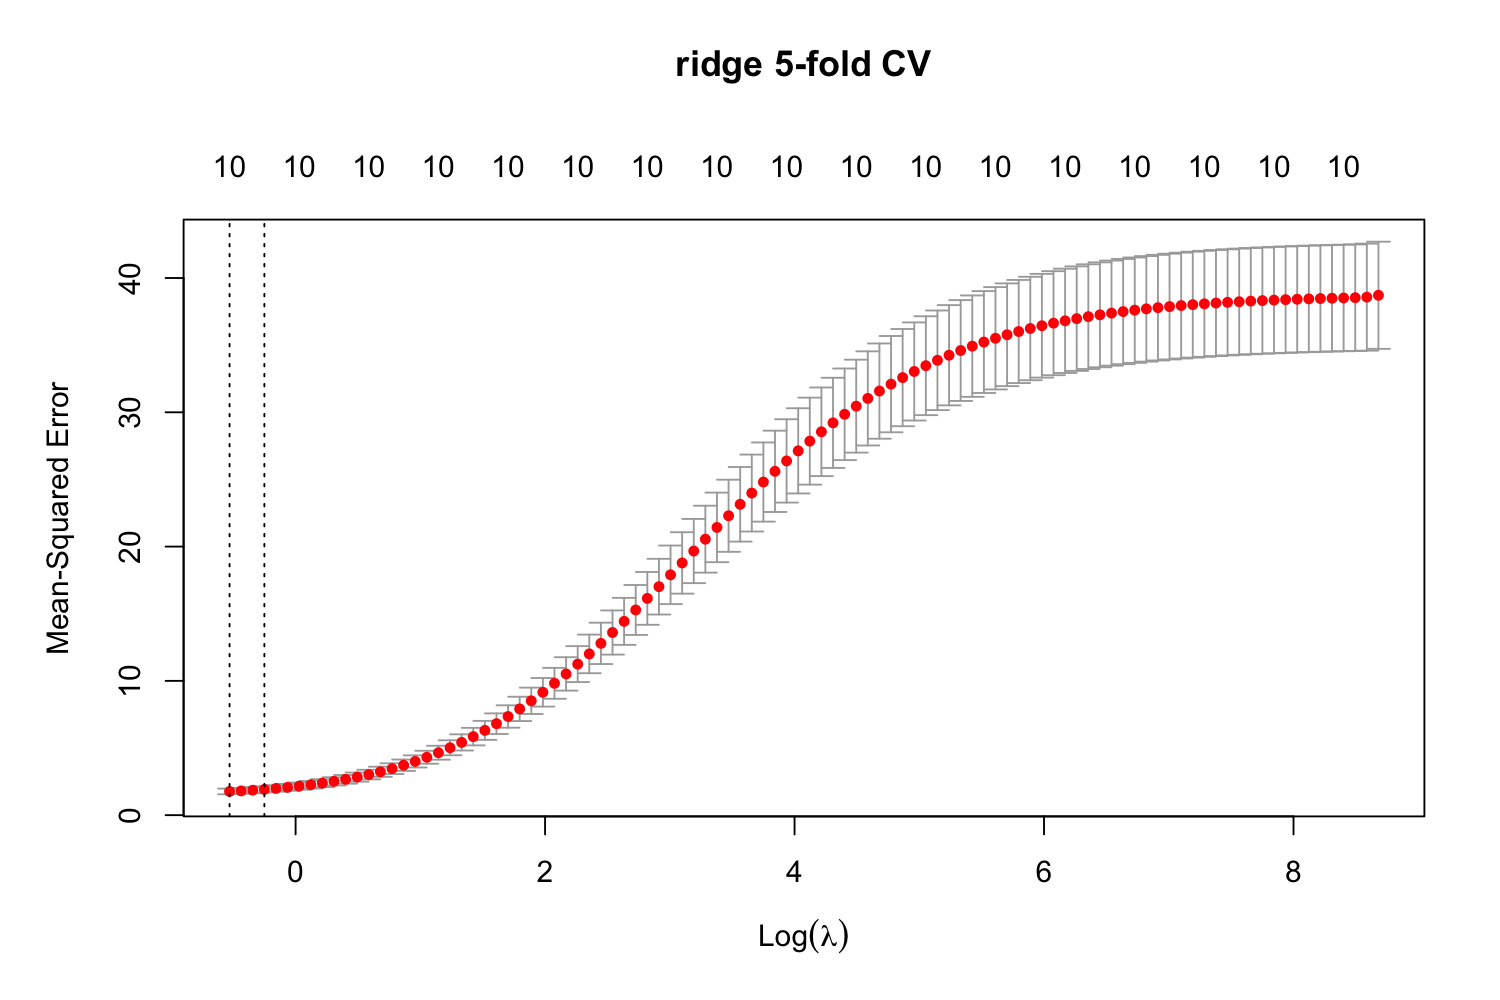
\includegraphics[width=0.85\linewidth]{assets/r-results/problem8-ridge-cv.png}
\end{center}
图中横轴为 $\log\lambda$，红点为验证集上平均 MSE；
两条竖虚线对应 \texttt{lambda.min} 与 \texttt{lambda.1se}，本题使用前者。

选定 $\lambda$ 后，提取全部 150 条训练记录拟合的系数。\texttt{coef()} 返回的系数已恢复到原始自变量量纲：
\begin{center}
\begin{tabular}{lr}
\toprule
变量 & 原始量纲系数 \\
\midrule
截距 & 1.036539 \\
Sex1 & 3.487333 \\
Ht & 0.001021 \\
Wt & 0.003990 \\
RCC & -0.188903 \\
WCC & 0.081993 \\
Hc & 0.008545 \\
Hg & -0.143324 \\
Ferr & 0.000762 \\
BMI & 0.124987 \\
SSF & 0.135335 \\
\bottomrule
\end{tabular}
\end{center}
将原始量纲的测试自变量传入 \texttt{predict()}，得到
$$
\mathrm{MSE}_{\mathrm{test,ridge}}
=\frac{1}{52}\sum_{i\in\mathrm{test}}(y_i-\hat y_i^{\mathrm{ridge}})^2
=1.234050
$$
\end{answerbox}

\subsection{}

拟合 lasso，报告同样结果及非零斜率的个数。比较两种方法的测试误差。（6 分）

\begin{answerbox}
\textbf{解：}

\begin{lstlisting}[style=rcode]
cv_lasso <- cv.glmnet(
  x_train, y_train, family = "gaussian", alpha = 1,
  foldid = foldid, nfolds = 5, type.measure = "mse",
  standardize = TRUE, intercept = TRUE
)
coef_lasso <- as.matrix(coef(cv_lasso, s = "lambda.min"))
pred_lasso <- as.numeric(predict(cv_lasso, newx = x_test, s = "lambda.min"))
mse_lasso <- mean((y_test - pred_lasso)^2)
\end{lstlisting}
令 $\alpha=1$，其余设置与岭回归一致，使用相同五折但独立选择 $\lambda$。得到
$$
\widehat\lambda_{\mathrm{lasso}}=0.1078180,\qquad
\mathrm{CV\ MSE}=1.402154.
$$
\begin{center}
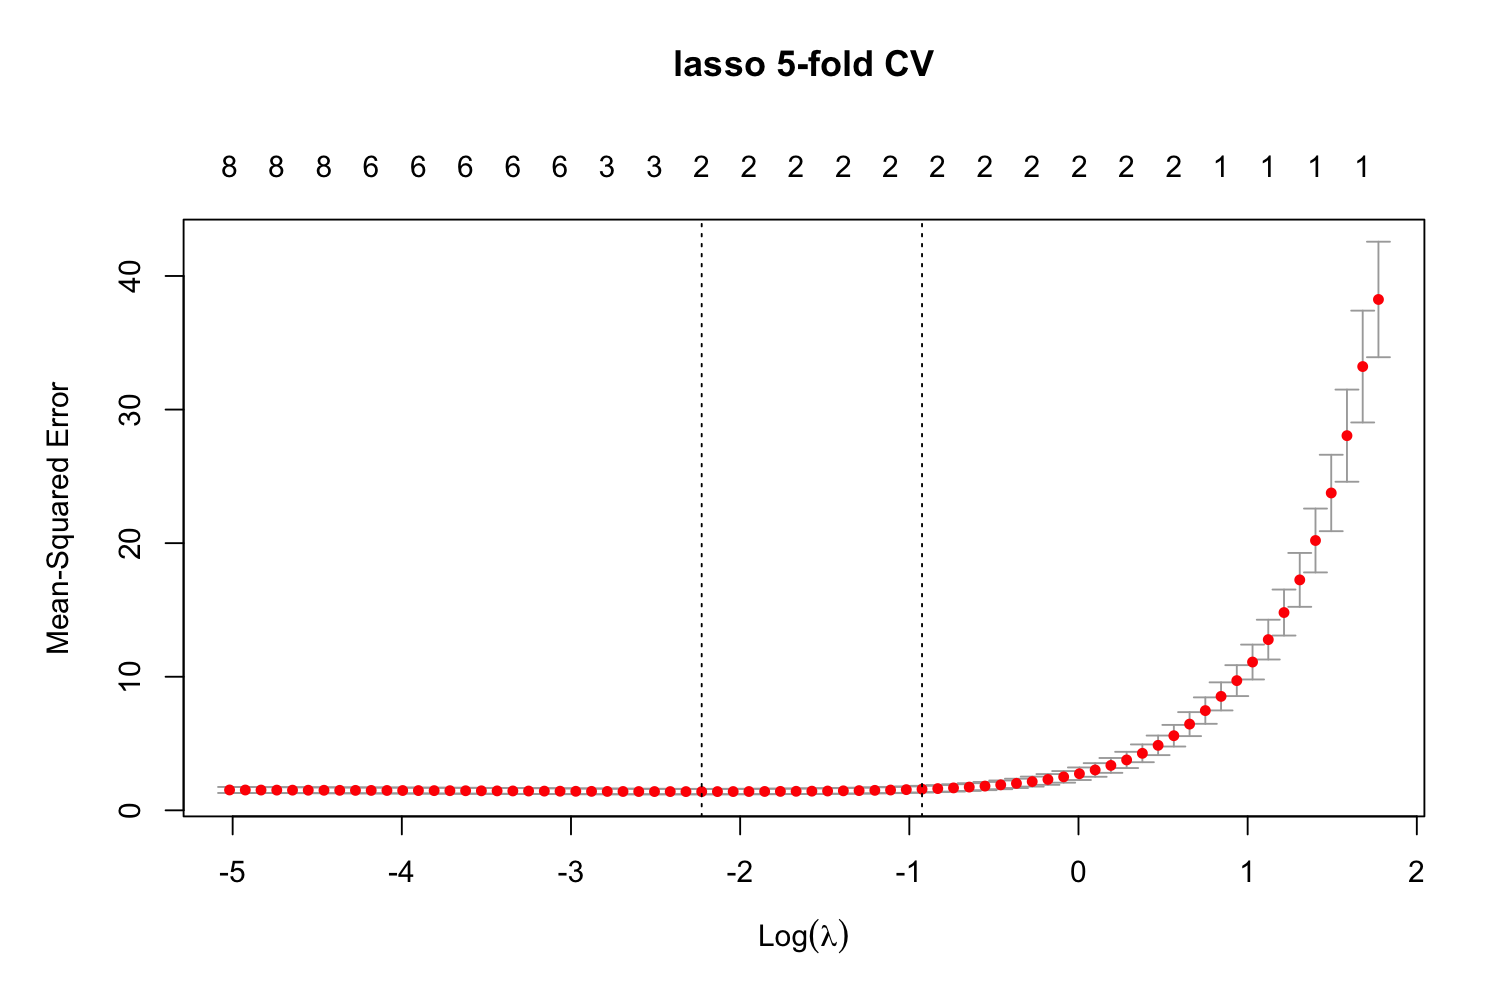
\includegraphics[width=0.85\linewidth]{assets/r-results/problem8-lasso-cv.png}
\end{center}
全训练集拟合的原始量纲系数为：
\begin{center}
\begin{tabular}{lr}
\toprule
变量 & 原始量纲系数 \\
\midrule
截距 & 1.240851 \\
Sex1 & 2.805359 \\
Ht & 0.000000 \\
Wt & 0.000000 \\
RCC & 0.000000 \\
WCC & 0.000000 \\
Hc & 0.000000 \\
Hg & 0.000000 \\
Ferr & 0.000000 \\
BMI & 0.000000 \\
SSF & 0.157284 \\
\bottomrule
\end{tabular}
\end{center}
非零斜率共 $2$ 个，分别为 \texttt{Sex1} 和 \texttt{SSF}，不计截距。预测方程为
$$
\hat y=1.240851+2.805359\,\mathrm{Sex1}+0.157284\,\mathrm{SSF}.
$$
测试误差为 $\mathrm{MSE}_{\mathrm{test,lasso}}=1.065576$，低于岭回归的 $1.234050$，相差约 $0.168474$。在本题指定划分下，Lasso 用更少的变量取得更低的测试误差。
\end{answerbox}

\subsection{}

在原始量纲上组合两种方法的预测：
\[
\hat{y}_i^{\mathrm{combo}}(\omega)=\omega\,\hat{y}_i^{\mathrm{ridge}}+(1-\omega)\,\hat{y}_i^{\mathrm{lasso}},\quad \omega=0,0.1,\dots,1.
\]
绘制测试 MSE 随 $\omega$ 的变化并描述结果；说明该曲线的最小值为何不能作为经独立测试验证的调参结果。若需要选择 $\omega$，应在哪个数据集上进行？（8 分）

\begin{answerbox}
\textbf{解：}
固定前两问通过训练集 CV 选出的模型，在原始响应量纲上计算加权预测。各权重对应的测试 MSE 如下：
\begin{center}
\begin{tabular}{rr}
\toprule
$\omega$ & 测试 MSE \\
\midrule
0.0 & 1.065576 \\
0.1 & 1.069947 \\
0.2 & 1.077091 \\
0.3 & 1.087008 \\
0.4 & 1.099696 \\
0.5 & 1.115158 \\
0.6 & 1.133391 \\
0.7 & 1.154397 \\
0.8 & 1.178176 \\
0.9 & 1.204727 \\
1.0 & 1.234050 \\
\bottomrule
\end{tabular}
\end{center}
\begin{center}
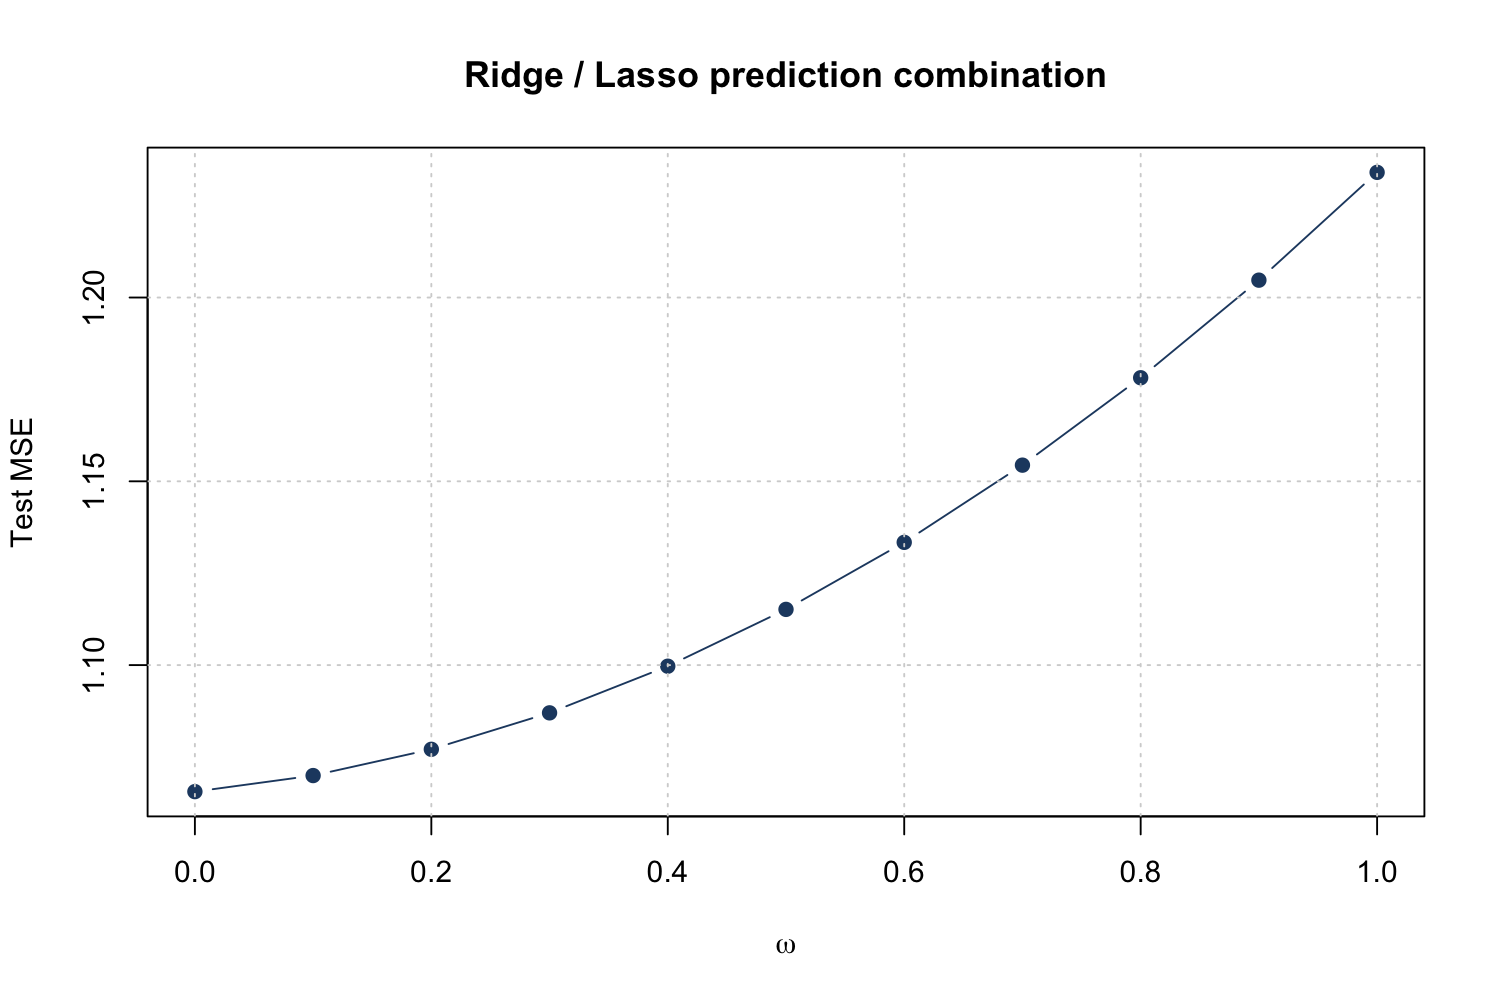
\includegraphics[width=0.85\linewidth]{assets/r-results/problem8-combo.png}
\end{center}
在给定网格上，测试 MSE 随 $\omega$ 增大而上升：$\omega=0$ 为纯 Lasso，误差最小，为 $1.065576$；$\omega=1$ 为纯岭回归，误差为 $1.234050$。本次测试样本上，混入岭回归预测没有降低误差。

该曲线可用于题目要求的事后描述，但若据其最小值选择 $\omega$，测试响应就参与了调参。同一测试集既用于选择权重又用于报告所选模型误差，便不再提供独立的最终评价，且可能产生选择带来的乐观偏差。

若需选择 $\omega$，应使用训练集内部的验证集或交叉验证预测，保留 52 条测试记录至所有参数固定之后。严格的交叉验证方案是在外层训练折中再选择两种模型的 $\lambda$，预测外层验证折，汇总折外预测后比较各 $\omega$ 的验证 MSE；选定权重后，用全部训练集重新拟合两种模型，最后仅在测试集评价一次。不能仅以查看测试曲线后选出的最小值声称组合模型已经得到独立验证。
\end{answerbox}

% ==================================================
\section{Problem 9（20 分）}

自学 group lasso，并用于 \texttt{ais.csv}。使用与第 8 题相同的因变量、训练/测试划分及五折编号，将十个自变量按以下顺序排列并分组：
\begin{center}
\begin{tabular}{ccl}
\toprule
组别 & 自变量 & 含义 \\
\midrule
1 & \texttt{Ht, Wt, BMI} & 身体尺寸 \\
2 & \texttt{RCC, Hc, Hg} & 红细胞相关指标 \\
3 & \texttt{WCC, Ferr} & 其他血液指标 \\
4 & \texttt{SSF} & 皮褶厚度 \\
5 & \texttt{Sex} & 性别（0/1） \\
\bottomrule
\end{tabular}
\end{center}
即 \texttt{groupid=c(1,1,1,2,2,2,3,3,4,5)}。请用训练集的均值及样本标准差标准化每一列（包括 \texttt{Sex}），并将同一变换应用于测试集。因变量保持原始量纲，截距不受惩罚，组惩罚权重取各组大小的平方根。按此训练集变换后的设计矩阵进行五折 CV；测试集不参与任何参数选择。可使用 R 包 \texttt{gglasso}（以下示例按 1.6 版，\texttt{L2} 对应均方误差）：
\begin{lstlisting}[style=rcode]
cv.gglasso(x, y, group=groupid, loss="ls",
  pred.loss="L2", foldid=foldid, nfolds=5)
gglasso(x, y, group=groupid, loss="ls", lambda=lambda)
predict(object, newx=x.test)
\end{lstlisting}
请报告软件包版本；使用其他版本时核对 \texttt{pred.loss} 的实际定义，确认用于调参的是平方预测误差；也可自行实现五折 MSE 验证。

\subsection{}

绘制 CV 误差曲线，用最小 CV MSE 选择 $\lambda$，报告截距、标准化量纲上的系数及保留的组。（12 分）

\begin{answerbox}
\textbf{解：}
使用 \texttt{gglasso} 1.6；已核对其 \texttt{cv.ls} 实现，\texttt{pred.loss="L2"} 先计算平方预测误差再取平均，对应本题要求的 MSE。

\textbf{数据与标准化。} 使用第 8 题相同的 150 条训练记录、52 条测试记录及训练集五折编号。
对每列 $j$，用训练集计算
$$
\bar x_j=\frac{1}{150}\sum_{i\in\mathrm{tr}}x_{ij},\qquad
s_j=\sqrt{\frac{1}{149}\sum_{i\in\mathrm{tr}}(x_{ij}-\bar x_j)^2},
\qquad z_{ij}=\frac{x_{ij}-\bar x_j}{s_j}.
$$
\texttt{Sex1} 也按此式标准化。测试集使用训练集的 $\bar x_j,s_j$，不使用测试数据估计变换。按题目约定，这里用全部 150 条训练记录估计变换，再在变换后的矩阵上分折，因此不能声称各轮的验证折完全没有参与标准化参数计算；这一操作与每折仅用 120 条拟合记录重新估计变换的流程不同。
因变量 \texttt{Bfat} 保持原始量纲。
\begin{lstlisting}[style=rcode]
vars9 <- c("Ht", "Wt", "BMI", "RCC", "Hc", "Hg",
           "WCC", "Ferr", "SSF", "Sex1")
x9_train_raw <- x_train[, vars9, drop = FALSE]
x9_test_raw <- x_test[, vars9, drop = FALSE]
mean9 <- colMeans(x9_train_raw)
sd9 <- apply(x9_train_raw, 2, sd)
x9_train <- scale(x9_train_raw, center = mean9, scale = sd9)
x9_test <- scale(x9_test_raw, center = mean9, scale = sd9)
y9_train <- y_train
y9_test <- y_test
foldid9 <- foldid
\end{lstlisting}


\textbf{模型与选参。} 令 $G_g$ 表示第 $g$ 组，$p_g$ 为组大小，最小化
$$
\frac{1}{2n_{\mathrm{tr}}}\sum_{i\in\mathrm{tr}}
(y_i-\beta_0-z_i^{\top}\beta)^2
+\lambda\sum_{g=1}^{5}\sqrt{p_g}\,\|\beta_{G_g}\|_2.
$$
五个组的惩罚权重为 $(\sqrt{3},\sqrt{3},\sqrt{2},1,1)$，截距不受惩罚。主要拟合代码为：
\begin{lstlisting}[style=rcode]
groupid <- c(1,1,1,2,2,2,3,3,4,5)
cv_group <- gglasso::cv.gglasso(
  x9_train, y9_train, group = groupid, loss = "ls",
  pred.loss = "L2", foldid = foldid9, nfolds = 5,
  pf = sqrt(as.numeric(table(groupid))), intercept = TRUE
)
lambda_group <- cv_group$lambda.min
coef_group <- coef(cv_group, s = "lambda.min")
\end{lstlisting}
使用软件自动生成的候选序列，选择平均验证 MSE 最小的 $\lambda$，得到
$$
\boxed{\widehat\lambda=0.09566076},\qquad
\min_{\lambda}\mathrm{CV\ MSE}=1.394610.
$$
\begin{center}
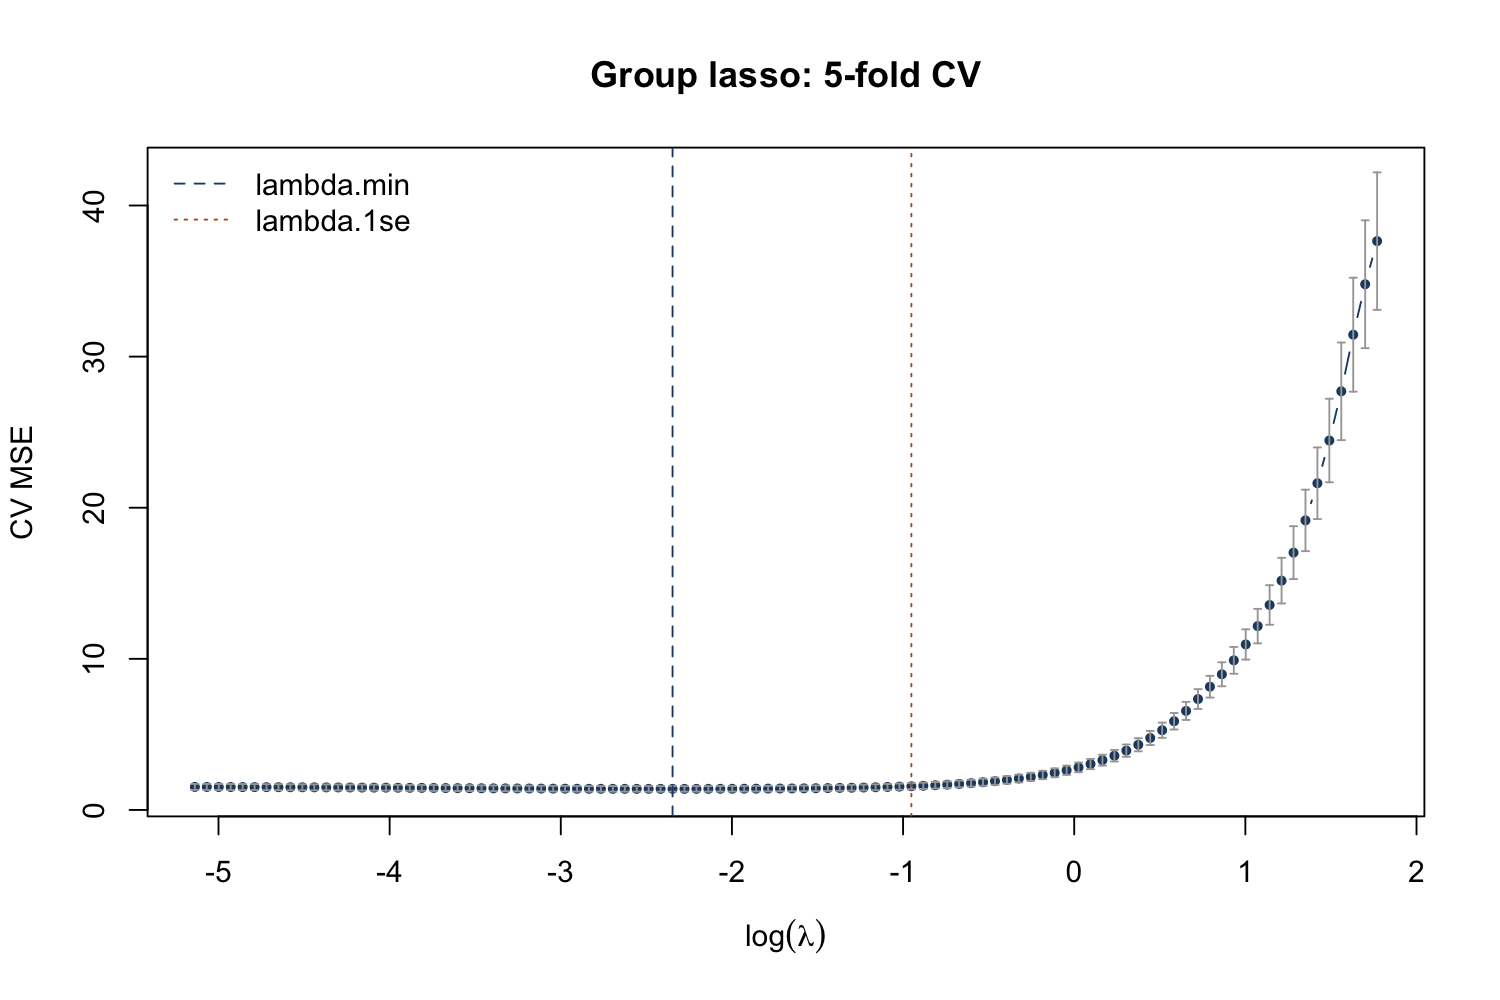
\includegraphics[width=0.85\linewidth]{assets/r-results/problem9-cv.png}
\end{center}
图中横轴为 $\log\lambda$，纵轴为 CV MSE，竖虚线标记 \texttt{lambda.min} 与 \texttt{lambda.1se}；本题采用 \texttt{lambda.min}。
另按相同候选序列逐折重算平方预测误差，整条曲线与软件输出的最大绝对差小于 $3\times10^{-14}$。

\textbf{系数与保留组。} 以下系数来自全部训练数据在选定 $\lambda$ 下的拟合，斜率对应标准化后的自变量 $z_j$：
\begin{center}
\begin{tabular}{lrr}
\toprule
变量 & 组别 & 标准化量纲系数 \\
\midrule
截距 & --- & 13.583667 \\
Ht & 1 & 0.000000 \\
Wt & 1 & 0.000000 \\
BMI & 1 & 0.000000 \\
RCC & 2 & 0.000000 \\
Hc & 2 & 0.000000 \\
Hg & 2 & 0.000000 \\
WCC & 3 & 0.000000 \\
Ferr & 3 & 0.000000 \\
SSF & 4 & 5.093761 \\
Sex1 & 5 & 1.415376 \\
\bottomrule
\end{tabular}
\end{center}
因此保留的组为 $G_4=\{\mathrm{SSF}\}, G_5=\{\mathrm{Sex1}\}$，第 1、2、3 组的系数整组为零。预测方程为
$$
\hat y=13.583667+5.093761\,z_{\mathrm{SSF}}
+1.415376\,z_{\mathrm{Sex1}}.
$$
这里的斜率不能直接与第 8 题的原始量纲系数比较；预测时必须使用训练集数据标准化后的 $z$。由于训练矩阵各列均值为零且截距不受惩罚，截距等于训练响应均值 $\bar y_{\mathrm{tr}}=13.583667$。
\end{answerbox}

\subsection{}

计算测试 MSE，与第 8 题比较；说明 group lasso 的组选择与普通 lasso 的变量选择有何不同。（8 分）

\begin{answerbox}
\textbf{解：}
使用训练集的均值和样本标准差变换测试自变量，并计算
\begin{lstlisting}[style=rcode]
pred_group <- as.numeric(
  predict(cv_group, newx = x9_test, s = "lambda.min")
)
mse_group <- mean((y9_test - pred_group)^2)
\end{lstlisting}
得到
$$
\mathrm{MSE}_{\mathrm{test,group}}
=\frac{1}{52}\sum_{i\in\mathrm{test}}(y_i-\hat y_i)^2
=\boxed{1.065165}.
$$
与第 8 题使用同一测试集的结果比较：
\begin{center}
\begin{tabular}{lrr}
\toprule
方法 & 测试 MSE & 非零斜率数 \\
\midrule
岭回归 & 1.234050 & 10 \\
普通 Lasso & 1.065576 & 2 \\
Group lasso & 1.065165 & 2 \\
\bottomrule
\end{tabular}
\end{center}
本次划分下，Group lasso 的测试 MSE 比普通 Lasso 低约 $0.000411$，两者非常接近，且都低于岭回归。仅凭这一次测试划分和如此小的差异，不能认为 Group lasso 具有稳定或显著的预测优势。各方法的 $\lambda$ 均由训练集 CV 决定，未使用测试误差调参。

普通 Lasso 的惩罚为 $\lambda\sum_j|\beta_j|$，以单个变量为单位产生稀疏性；即使几个变量属于同一组，也可以只保留其中部分变量。Group lasso 的惩罚为 $\lambda\sum_g\sqrt{p_g}\|\beta_{G_g}\|_2$，以整组系数向量为选择单位：若 $\|\beta_{G_g}\|_2=0$，该组所有变量同时删除；若组范数非零，则该组被保留。其组内 $L_2$ 惩罚通常不产生逐变量稀疏性，但不能据此断言保留组内每个系数必然非零。

本题中两种方法恰好都保留 \texttt{SSF} 与 \texttt{Sex1}，而这两个组都只含一个变量，其组范数即系数绝对值。因而当前结果没有展示多变量组被保留的情形。
一般情况下，两种方法的惩罚单位不同，选择结果不必相同。
\end{answerbox}

\begin{center}
{\color{linegray}\rule{0.9\textwidth}{0.8pt}}\\[0.5em]
{\small\color{textgray} 参考：\url{https://cran.r-project.org/web/packages/gglasso/gglasso.pdf}}
\end{center}

\end{document}
